% Tento soubor nahraďte vlastním souborem s obsahem práce.
%=========================================================================
% Autoři: Michal Bidlo, Bohuslav Křena, Jaroslav Dytrych, Petr Veigend a Adam Herout 2019

% Pro kompilaci po částech (viz projekt.tex), nutno odkomentovat a upravit
%\documentclass[../projekt.tex]{subfiles}
%\begin{document}

\chapter{Úvod}
Zlepšení finanční gramotnosti v~České republice je stále téma, které mnoho odborníků neví jak řešit. Moje motivace není v~celkovém řešení společenského problému, nýbrž chci přivést na trh nástroj, který dokáže pomoci běžnému občanu České republiky v~každodenním rozhodování o~jeho financích. Sestavením rodinného rozpočtu se zabývám několik posledních let a~tato zkušenost mě přivedla k~vytvoření této práce a~pomoci nejen sobě, ale i~ostatním v~oblasti finanční zodpovědnosti. Zároveň zde mohu zúročit, vše co mě naučila vysoká škola v~oblasti umělé inteligence a~programování webových aplikací.

Proto jsem se rozhodl vytvořit tuto práci a~vytvořit nekomerční řešení pro správu rodinných financí.

Cílem této bakalářské práce je vytvořit webovou aplikaci, která bude analyzovat transakce
a~řadit je do předem určených kategorií. Po registraci uživatelovi tato aplikace dovolí nahrát své měsíční bankovní výpisy. Uživatel si vybere svou bankovní společnost, díky které se aplikuje šablona formátu výpisu na jeho formát.

Následně se extrahují jednotlivé transakce a~pomocí umělé inteligence se roztřídí do různých obecných kategorií, např. jídlo, transport, potraviny a~energie. Následně se tyto transakce zobrazí v~přehledném grafu s~informacemi, ve které sekci má nejvyšší výdaje. 
Součástí aplikace bude také ruční úprava transakcí, pokud umělá inteligence špatně zvolí kategorii nebo nedokáže sama tuto kategorii zařadit. Uživatel může i~ručně odebírat transakce a~prohlížet si grafy z~minulých měsíců. Aplikace si bude zakládat na uživatelské přívětivosti a~jednoduchosti používání.

V~první kapitole shrnu a~rozeberu současné aplikace na trhu a~důvody, proč vytvářím aplikaci novou. Každou aplikaci shrnu v~pár větách a~zdůvodním její nedostatky.

Prvním bodem mého zadání bylo se seznámit s~problematikou vytváření webových aplikací. Součástí je i~následné vyhodnocení a~výběr vhodného frameworku a~architektury, která bude použita pro realizaci výsledné aplikace.

V~další kapitole se seznámíme s~dostupnými formáty výpisů, které poskytují přední bankovní instituce v~České republice a~provedu analýzu požadavků pro naši aplikaci pomocí diagramu případů užití.

Druhým bodem je analýza popisu transakcí a~extrakce údajů. Tato data poté využijeme na kategorizaci transakcí umělou inteligencí. Následujícím krokem je sestavení vhodného modelu pro umělou inteligenci a~jeho následné trénování na testovacích datech.

Třetí část souvisí s~návrhem výsledné aplikace a~s~tímto bodem také spojená tvorba ER diagramu. Detailně zde bude popsán návrh uživatelského rozhraní a~API.

V~následující části uvedu, jak vypadá implementace samotné aplikace a~rozeberu automatickou klasifikaci transakcí.
V~předposlední kapitole shrnu výsledky testování celé aplikace a~vyzkouším aplikaci testováním na několika lidech.

V~poslední kapitole shrnu výsledky práce, zmiňuji se i~o~její použitelnosti a~také o~možnostech pro její budoucí rozvoj.

\chapter{Analýza průzkumu trhu}
V~následující kapitole budou popsány nejznámější aplikace pro správu financí. 
\section{Mobilní aplikace}
V~dnešní době jsou mobilní aplikace důležitější a~rozšířenější, než kdy dříve. V~oblasti financí jsou mobilní aplikace stále důležitější pro uživatele, kteří chtějí být informováni o~stavech na bankovních účtech a~plánovat své výdaje. Trh s~mobilními aplikacemi, které se zabývají rozpočtem je opravdu obrovský, každá umí něco jiného a~má svá specifika, jak ji používat.
\subsection*{Spendee}
Nejoblíbenější aplikací na trhu je aplikace Spendee\footnote{\url{https://www.spendee.com/}}. Aplikace dokáže sledovat vaši útratu pomocí propojení na bankovní API. Jako jediná aplikace se dokáže napojit i~na české banky. Tato služba zní velmi zajímavě bohužel její hlavní nevýhoda je, že je placená. Měsíční předplatné stojí buď 2\$ nebo dražší 3\$. Aplikace je na trhu již od roku 2018. Spendee nabízí uživatelům také přehledné statistiky o~jejich výdajích a~příjmech. Aplikace zobrazuje grafy a~tabulky, které umožňují uživatelům vidět, jak se stav jejich financí vyvíjí v~průběhu času. Díky tomu mohou uživatelé lépe plánovat své budoucí výdaje a~sledovat, jak se jim daří hospodařit s~penězi. Aplikace cílí na masovou společnost, která chce jednoduché ovládání a~pěkné barevné GUI. Během testování jsem zaznamenal problémy s~propojením s~Komerční bankou, kdy aplikace často přerušovala spojení. Spendee je určitě skvělou volbou pokud chceme sledovat naše finance a~nevadí nám časté přihlašování do bankovního API. Rozhraní aplikace můžeme vidět na obrázku \ref{fig:speende1} a~rozvržení grafu na obrázku \ref{fig:speende2}.

\begin{figure}[H]
  \centering
  \begin{minipage}[b]{0.4\textwidth}
    \includegraphics[height=10cm]{spendeecropped.pdf}
    \caption{Aplikace Spendee souhrn výdajů.}
    \label{fig:speende1}
  \end{minipage}
  \hfill
  \begin{minipage}[b]{0.4\textwidth}
    \includegraphics[height=10cm]{obrazky-figures/spendee1.pdf}
    \caption{Aplikace Spendee souhrn graf.}
    \label{fig:speende2}
    
  \end{minipage}
\end{figure}
\subsection*{YNAB (You need a~budget)}

YNAB\footnote{\url{https://www.ynab.com/}} (You Need A~Budget) je aplikace pro správu osobních financí, která pomáhá uživatelům získat kontrolu nad svými financemi a~plánovat své výdaje. Tato aplikace se zaměřuje na tzv. pravidlo 4 kroků, které zní:
\begin{itemize}
    \item Přiřazuj každý dolar k~nějakému výdaji.
    \item Sleduj všechny výdaje.
    \item Stanov si priority pro výdaje.
    \item Zůstávej v~mezích svého rozpočtu.
\end{itemize}
YNAB pomáhá uživatelům žít podle svého rozpočtu a~plánovat si své výdaje s~předstihem, což umožňuje snížit stres z~financí a~dosáhnout finanční svobody.
Aplikace stojí 15\$ měsíčně a~nemá žádnou neplacenou verzi. Do aplikace si postupně zapíšete svoje měsíční výdaje a~následně vás aplikace požádá o~doplnění transakcí. Aplikace také nabídne napojení na API banky, ale v~seznamu se nenachází žádná česká banka. Aplikace umožní nahrání CSV souboru pouze přes webové prostředí, které je značně nepřehledné a~je nutné upravit CSV soubor, který nám poskytne banka. Na obrázku \ref{fig:ynab} můžeme vidět modální okno pro nahrání souboru.
\begin{figure}[ht]
    \centering
    \includegraphics[width=\textwidth]{obrazky-figures/ynab.png}
    \caption{Nahrávání výpisu do YNAB.}
    \label{fig:ynab}
\end{figure}
\section{Webové aplikace}

Webové aplikace jsou programy, které běží v~internetovém prohlížeči uživatele a~umožňují interakci s~obsahem na internetu. Tyto aplikace jsou stále populárnějšími, neboť jsou snadno dostupné, nemusí se instalovat a~mohou být používány na jakémkoli přístroji s~připojením k~internetu. Ve světě financí si lidé zvykli na internetové bankovnictví. Byla to první možnost komunikace s~bankou bez bankéře a~lidé je používají i~dnes, a~právě proto si myslím, že v~dnešní době dává smysl mít finanční aplikace dostupné na webu.

\subsection{Mint}
Aplikace Mint\footnote{\url{https://mint.intuit.com/}} je nástroj pro správu financí, která slouží ke sledování a~správě vašich osobních financí. Tato aplikace vám umožňuje propojit vaše bankovní účty, kreditní karty, investiční účty a~další finanční účty, aby vám poskytla celkový přehled o~vašich finančních aktivitách. Mint vám umožňuje sledovat vaše příjmy a~výdaje, kategorizovat transakce a~sledovat vaše výdaje v~reálném čase. Aplikace vám také poskytuje různé nástroje a~funkce, např. upozornění na zůstatek na účtu, sledování kreditního skóre, plánování rozpočtu a~investiční nástroje. Webová aplikace není dostupná v~České republice, nepodporuje banky působící na tuzemském trhu, ale v~zahraničí je velmi oblíbená, podobně jako Spendee. Také zde přidáváme své transakce po jedné a~následně vidíte grafy, kde se co dá zlepšit. Aplikace působí přehledně.

\subsection{Goodbudget}
Goodbudget\footnote{\url{https://goodbudget.com/}} je aplikace pro správu osobních financí, která pomáhá uživatelům plánovat své výdaje pomocí obálkové metody. Tato metoda spočívá v~tom, že uživatelé si přiřadí k~jednotlivým kategoriím své výdaje do obálky s~určitými peněžními limity a~snaží se tyto limity nepřekročit. Goodbudget umožňuje uživatelům sledovat, kolik peněz jim zbývá v~každé kategorii, a~tím koordinovat následující výdaje. Aplikace také umožňuje sdílet účty s~rodinou.
Webová aplikace nabízí jednoduché nahrání CSV souboru, dokonce ve webovém prostředí nabídne úpravu CSV souboru. Moje testovací výpisy z~Komerční banky, ale byly velmi špatně rozpoznány a~ani v~jedné transakci nebyla správná hodnota transakce, jak můžeme vidět na obrázku \ref{fig:goodbudget}
\begin{figure}[ht]
    \centering
    \includegraphics[width=\textwidth]{obrazky-figures/goodbudget.png}
    \caption{Přehled transakcí v~Goodbudget.}
    \label{fig:goodbudget}
\end{figure}

\section{Závěr}
Shrnul jsem zde 4 aplikace pro správu osobních financí, které jsou v~dnešní době dle různých internetových magazínů nejpopulárnější a~také jsem si je mohl osobně vyzkoušet. Největší negativa těchto aplikací jsou uživatelská nekomfortnost při nahrávání vašich výpisů a~placení měsíčních poplatků. Z~této analýzy jsem dospěl k~závěru, že v~České republice chybí nekomerční aplikace pro kategorizaci vašich výdajů.

\chapter{Použité technologie}
V~této kapitole budou prezentovány informace o~použitých technologiích při vývoji aplikace a~důvody pro volbu daných technologií.
\section{Webové frameworky}

Dny, kdy se weby psaly pouze v~HTML a~CSS jsou již za námi. Ani s~přidaným Javascriptem na rozpohybování HTML elementů, již dnes plnohodnotnou webovou aplikaci nenapíšeme jednoduše. Z~webů se staly robustnější aplikace tzv. webové aplikace, které potřebují složitější logiku a~tak vznikly webové frameworky.

Webové technologie jsou jedny z~nejrychleji vyvíjejících technologií v~oblasti informačních technologií. Webové aplikace jsou v~podstatě aplikace na architektuře klient--server, kterou si popíšeme později. Běží ve webovém prohlížeči a~komunikují přes protokol HTTP. Novým standardem pro webové aplikace se staly webové frameworky, které nám ulehčují jejich vývoj.

\subsection{Single--page weby}
Single--page aplikace je webová aplikace, jejíž veškerý obsah je tvořen jedinou stránkou. Uživatel této aplikace nemusí po každém kliknutí na nový obsah stránky stahovat celou stránku znovu, stačí pouze načíst obsah, který potřebujeme obnovit~\cite{barborakoouskov_2020_co}.
Single--page aplikace se v~dnešní době dělají pomocí javascriptových frameworků a~knihoven. Na obrázku \ref{graf:stack} můžeme vidět 6 nejvyhledávanějších a~nejvyužívanějších webových frameworků v~roce 2022~\cite{stackoverflow}:

\begin{figure}[H]
    \centering
    \includegraphics[width=\textwidth]{obrazky-figures/table1.png}
    \caption{Popularita webových frameworků v~roce 2022 \cite{stackoverflow}.}
    \label{graf:stack}
\end{figure}
Všechny si postupně rozebereme v~následujících kapitolách.
\subsection{Node.js}
Node.js\footnote{\url{https://nodejs.org/en}} umožňuje programátorům používat JavaScript na straně serveru, což znamená, že lze vytvářet komplexní webové aplikace pomocí jediného jazyka -- JavaScriptu~\cite{mal_2010_nodejs}. Node.js je ideální pro tvorbu rychlých, škálovatelných a~vysoce výkonných webových aplikací, API nebo serverových služeb~\cite{barborakoouskov_2020_pro}. V~předchozích letech Node.js nebyl považován za webový framework, ale v~dnešní době ho již mnoho vývojařů považuje za plnohodnotný framework a~tvoří základ pro vytváření dalších webových frameworků, jako například Express.js, který poskytuje další vrstvu abstrakce. V~mé práci by volba Node.js dávala smysl pouze při volbě jazyka JavaScript pro serverovou část aplikace.

\subsection{React.js}
React.js\footnote{\url{https://react.dev/}} je javascriptová knihovna pro tvorbu uživatelského rozhraní. Vytvořena byla zaměstnancem firmy Facebook a~je dále rozvíjena firmou Meta (dříve Facebook)~\cite{fedosejev2015react}. Hlavní výhodou a~také důvodem, proč v~této práci bude použit React je virtuální DOM (Document Object Model), díky kterému může aplikace rychle reagovat na změny v~datovém modelu a~držet přitom stabilní výkon aplikace. Další skvělou výhodou je jedna z~největších komunitních základen a~rozsáhlá dokumentace. Správa stavů a~synchronizace aplikace s~datovým modelem je zde implementována přívětivě.

\subsection{jQuery}
jQuery\footnote{\url{https://jquery.com/}} je javascriptová knihovna s~širokou podporou prohlížečů, která klade důraz na interakci mezi JavaScriptem a~HTML. Byla vytvořena v~roce 2006\footnote{\url{https://blog.jquery.com/2006/08/26/jquery-10/}} a~jedná se tak o~nejstarší knihovnu v~našem výběru a~hlavně kvůli stáří ji nechci ve své práci používat.

\subsection{Express}
Express\footnote{\url{https://expressjs.com/}} je populární open--source framework pro Node.js, který umožňuje vytvářet webové aplikace a~API. Express poskytuje jednoduché a~minimalistické rozhraní pro vytváření serverových aplikací. Express je serverový javascriptový framework a~protože bude náš server hodně pracovat s~úpravou dat Javascript není úplně správná volba, proto ho nebudeme v~naší práci používat.

\subsection{Flask}
Flask\footnote{\url{https://flask.palletsprojects.com/en/2.2.x/}} je open--source webový framework pro programování webových aplikací v~jazyce Python. Je to lehký framework, který nabízí jednoduchou a~elegantní architekturu, což umožňuje programátorům rychle a~snadno vytvářet webové aplikace. 
Mezi výhody použití Flasku patří jeho jednoduchá architektura, která umožňuje programátorům rychle se s~ním seznámit a~začít s~vývojem webových aplikací. Flask také umožňuje rozšiřování a~přizpůsobení podle potřeb vývojářů, což z~něj činí vhodný framework pro malé a~střední webové projekty. Flask také obsahuje rozsáhlou dokumentaci a~silnou komunitu, což umožňuje vývojářům rychle najít řešení problémů. V~naší aplikace bude Flask běžet na serveru a~díky jazyku Python nám umožní zprovoznění umělé inteligence přes knihovnu PyTorch. Python je též skvělý a~použitelný pro dolování z~dat a~práci s~řetězcem textu.

\subsection{Angular}
Angular\footnote{\url{https://angular.io/}} je open--source webový framework vyvíjený společností Google, který slouží k~vývoji moderních a~dynamických webových aplikací. Angular využívá jazyk TypeScript, který umožňuje psát kód s~větší jistotou, což zlepšuje jeho čitelnost a~údržbu.
Mezi nevýhody použití Angularu patří jeho složitější syntaxe, která může být pro programátory náročná. Angular také vyžaduje větší množství zbytečného kódu a~konfigurace než jiné webové frameworky, což může vést k~většímu objemu kódu a~zvýšené složitosti aplikace. 

\subsection{Vue.js}
Vue.js\footnote{\url{https://vuejs.org/}} je moderní a~open--source frontendový framework pro vývoj webových aplikací a~uživatelských rozhraní (UI). Byl vytvořen v~roce 2014 a~jeho hlavním tvůrcem je Evan You\footnote{\url{https://vuejs.org/about/faq.html}}. Jeho cílem je poskytnout jednoduchý a~flexibilní framework pro vývoj moderních webových aplikací. Hlavní nevýhodou tohoto frameworku je malá komunita, což může vést k~menšímu počtu návodů, knihoven a~rozšíření.

\section{Architektura}
Správná architektura webové aplikace může výrazně ovlivnit úspěch a~celkovou kvalitu aplikace. Tím pádem je důležité pečlivě zvážit při návrhu architektury webové aplikace různé faktory jako jsou potřeby uživatelů, požadavky na výkon a~škálovatelnost, zabezpečení a~další. Celá architektura je postavena na konceptu Třívrstvé architektury. Následující kapitola je převzata z~\cite{rouse_2021_threetier}.
\subsection{Třívrstvá architektura}
Je to metoda rozdělení architektury aplikace do tří nezávislých vrstev -- prezentační, aplikační a~datová. Každá má svůj specifický úkol. Na obrázku \ref{fig:trivstva} můžete vidět diagram propojení celé architektury.


\begin{figure}[ht]
\centering
\includegraphics[width=\textwidth]{./obrazky-figures/server_klient.pdf}
\caption{Třívrstvá architektura.}
\label{fig:trivstva}
\end{figure}

\subsubsection{Prezentační vrstva}
Jediná vrstva se kterou interaguje uživatel, ten zadá vstupní data a~zobrazí se mu výstupní data ve srozumitelné formě. Zahrnuje různé typy UI prvků, jako jsou formuláře, tlačítka, seznamy, tabulky a~další. Tyto prvky umožňují uživatelům zadávat data, procházet seznamy a~zobrazovat výsledky svých akcí. Prezentační vrstva má také vliv na celkový vzhled a~pocit z~aplikace. Vývojáři musí zvážit různé faktory, jako jsou typy uživatelů, účel aplikace, obecné návyky uživatelů a~další faktory, při navrhování uživatelského rozhraní. V~dnešní době se také klade důraz na přístupnost a~zohlednění přístupu pro lidi s~nějakým postižením. Prezentační vrstva je zastoupena v~mé práci klientem a~bude implementována frameworkem React.js.
\subsubsection{Aplikační vrstva}
Tato vrstva má na starosti logiku celé aplikace a~stará se o~zpracování dat. Přijímá požadavky prezentační vrstvy a~ty dále zpracovává. Hlavním úkolem aplikační vrstvy je zpracování požadavků uživatelů. Aplikační vrstva je v~mé práci zastoupena serverem a~bude implementována frameworkem Flask. V~této vrstvě bude probíhat kategorizace transakcí pomocí modelu umělé inteligence s~knihovnou PyTorch.
\subsubsection{Datová vrstva}
Datová vrstva je nejnižší vrstva architektury, která se stará o~ukládání a~získávání dat z~databáze. Hlavním úkolem datové vrstvy je zajistit, aby data byla ukládána bezpečně, konzistentně a~efektivně, a~aby byla snadno dostupná pro další zpracování v~aplikaci. Správná funkčnost datové vrstvy je zásadní pro celkovou funkčnost aplikace, protože zajišťuje, že data jsou uložena a~zpracována správným způsobem. V~této vrstvě budu používat MariaDB.
\subsection{Server}
Na serveru budu využívat webový framework Flask, který nabízí celou řadu užitečných funkcionalit, včetně efektivní práce s~textovými řetězci a~schopnosti stavět API ve formě logických celků. Python disponuje rozsáhlou knihovnou funkcí a~modulů jako např. knihovnu pro práci s~umělou inteligencí PyTorch.
\subsection{Klient}
Pro klienta budu využívat webový framework React. Vybral jsem si jej zejména díky komunitní základně a~využití virtuálního DOM modelu, který se bude hodit při tvorbě aplikace a~zjednoduší některé činnosti. Díky propojení přes API nemusím řešit žádnou kompatibilitu mezi frameworky na serveru a~klientu.
\subsection{Databáze}
Správná volba databázového systému je klíčová pro úspěšné dokončení projektu. MariaDB\footnote{\url{https://mariadb.com/}} je relační databázový systém, který vznikl v~roce 2009 jako fork MySQL\footnote{\url{https://www.mysql.com/}}, a~díky svým vlastnostem a~výhodám si získal popularitu mezi uživateli i~vývojáři. Je to open-source software s~velkou komunitou uživatelů a~vývojářů, což umožňuje uživatelům upravovat a~rozšiřovat systém podle svých potřeb. MariaDB má silnou reputaci na trhu databázových systémů. MariaDB obsahuje několik vylepšených funkcí, které nejsou v~MySQL k~dispozici např. pokročilé dotazy, lepší indexování, optimalizaci dotazů, nové úložiště pro datové typy a~další~\cite{mariadb}.

\section{Síťová komunikace}
V~následující části budu popisovat, jakými protokoly a~formáty server a~klient komunikují mezi sebou. Přenos dat je šifrován přes HTTPS, data se posílají ve formátu JSON.
\subsection{HTTP}
HTTP (Hypertext Transfer Protocol) je protokol aplikační vrstvy. Dnes je hlavně používaný na přenos dat po síti. Základní princip tohoto protokolu je odesílání požadavku a~očekávání odpovědi ze serveru. Protokol si neukládá jednotlivé požadavky, to značí že je bezstavový~\cite{a2021_ibm}. Bezstavovost budeme řešit pomocí autentizačních hlaviček s~tokeny. 
\subsubsection{Základní HTTP metody}
HTTP metody jsou používány k~určení, jakým způsobem bude zpracován požadavek odeslaný klientem na server. Při odesílání na adresu se přidávají k~metodám také informace o~verzi protokolu a~různé hlavičky. Existují čtyři základní metody~\cite{gourley2002http}:
\begin{itemize}
\item \texttt{GET} -- Odesílá požadavek na získání informací na serveru.
\item \texttt{POST} -- Odesílá informace, které mají být zpracovány na serveru.
\item \texttt{PUT} -- Odesílá kompletní zdrojový soubor na server.
\item \texttt{DELETE} -- Odesílá informace, které se mají smazat na webovém serveru.
\end{itemize}
Dále existují také další metody, jako např. \texttt{HEAD}, \texttt{OPTIONS}, \texttt{TRACE} nebo \texttt{CONNECT}, které se používají v~speciálních případech, v~mé práci nebudou potřeba.
Při přijímání odpovědi na požadavek dostáváme odpověď ve formě číselného kódu:
\begin{itemize}
    \item 1xx -- informační charakter,
    \item 2xx -- operace schválena, akceptována,
    \item 3xx -- operace přesměrování, potřeba dalších úprav pro splnění požadavku,
    \item 4xx -- operaci nelze splnit,
    \item 5xx -- chyba na straně serveru,
\end{itemize}

\subsection{HTTPS}
HTTPS (Hypertext Transfer Protocol Secure) je rozšíření již uvedeného aplikačního protokolu HTTP. Hlavní nevýhoda původního protokolu byla možnost sledování a~čtení komunikace mezi serverem a~klientem a~takovou vlastnost u~aplikace zaměřenou na finance nechceme.
U~HTTPS jsou použity kryptovací protokoly s~asymetrickým šifrováním. Toto šifrování chrání komunikaci mezi klientem a~server. Tato technologie zabraňuje podvržení zpráv i~jejich čitelnost někým jiným než serverem a~klientem, kteří mezi sebou tuto komunikaci vedou~\cite{rfchttps}.

\subsection*{Application Programming Interface}

API (Application Programming Interface) je komunikační rozhraní, které používají webové služby pro komunikaci mezi servrem a~klientem.
API jednoznačně odděluje prezentační část od aplikační a~dovoluje napojit webovou i~mobilní aplikaci pomocí stejného rozhraní.
Mezi nejpoužívanější architekturu patří REST.
\subsubsection{REST API}
REST (Represational State Transfer) komunikuje prostřednictvím protokolu HTTP. Díky tomu může využívat již implementované hlavičky, metody, tělo a~stavové kódy. Základní HTTP metody (GET, POST, PUT a~DELETE) se přetransformují na CRUD (Create, Read, Update a~Delete) operace, které zprostředkuje server~\cite{restapibook}:
\begin{itemize}
\item \texttt{POST} $\rightarrow$ Create -- Odesílá požadavek na vytvoření dat.
\item \texttt{GET} $\rightarrow$ Read -- Posílá zpátky informace o~datech.
\item \texttt{PUT} $\rightarrow$ Update -- Odesílá požadavek na úpravu dat.
\item \texttt{DELETE} $\rightarrow$ Delete --  Odesílá požadavek na smazání dat.
\end{itemize}
REST architektura má obecně definované principy~\cite{restapibook}, které jsem se snažil dodržet v~mé práci:
\begin{itemize}
    \item Jednotné rozhraní
    \item Architektura klient--server
    \item Bezstavová logika
    \item Vrstvená architektura
    \item Kód na vyžádání
    \item Ukládání dat do cache
\end{itemize}

\subsection{JSON}
JSON (JavaScript Object Notation) je formát pro přenos dat. Jeho syntaxe je založena na JavaScriptových objektech a~polích a~umožňuje reprezentovat data ve formátu hierarchických stromů. Data jsou uloženy ve formátu \texttt{\{"klíč":"hodnota"\}}. Tento formát je čitelný jak pro stroje, tak i~pro lidské oko~\cite{rfcjson}.

\section{Autentizace}
Autentizace neboli ověření uživatelovy identity lze provádět mnoha způsoby. V~mé aplikaci jsem zvolil klasický způsob ověření, a~to přes uživatelův email a~heslo. Tento email bude pro každého uživatele taktéž jedinečný identifikátor. Kromě tohoto klasického způsobu se stále více využívá biometrie, díky její rychlosti a~přesnosti. U~bankovních aplikací jsou také rozšířené PIN kódy, bezpečnostní kódy a~nebo osobní otázky. V~rámci zvýšení zabezpečení může společnost používat i~více druhů autentizace a~tak zvýšit bezpečnost na úkor uživatelské přívětivosti~\cite{dasgupta2017advances}.

\subsection*{JWT token}
JWT (JSON Web Token) je internetový standard pro formát tokenu, který lze použít pro autentizaci a~autorizaci. 
Jedná se o~kompaktní a~samostatně přenositelný způsob přenosu informací o~uživateli mezi různými částmi aplikace. JWT obsahuje zakódované informace o~uživateli v~JSON formátu, které jsou podepsané digitálním podpisem pro zajištění integrity dat~\cite{rfc7519}.
Po autentizaci se vytvoří na serveru token (API endpointem \texttt{/token}), který pomocí API rozhraní přijme prohlížeč a~uloží si ho do Local Storage. Local Storage (Web Storage) je jedna z~funkcionalit moderních webových prohlížečů, která dovoluje aplikacím ukládat data na počítači uživatele. Tato data se ukládají přímo do paměti prohlížeče a~jsou k~dispozici i~po restartu prohlížeče~\cite{shwetank_2013_web}. Při každém dalším volání API se do HTTP hlavičky přidá řádek s~autentizačním tokenem. Tak server pozná o~jakého uživatele se jedná a~podle toho uzpůsobí dál svoje chování.


\chapter{Analýza požadavků}
V~následující kapitole budou popsány jaké formáty bankovní společnosti nabízejí.
\section{Formáty souborů bank}
\label{chap:formaty}
Při zkoumání výpisů formátu aplikace jsem kontaktoval všechny přední banky v~České republice formou telefonického hovoru nebo emailem a~zeptal jsem se, jaké formáty nabízí pro výpisy. Základním formát souboru je PDF, ten nabízí všechny bankovní společnosti. Tento formát se velmi špatně čte z~pohledu automatizovaného procesu programem. Strojově čitelné formáty pro programy jsou třeba CSV nebo XML. Dle mého průzkumu minimálně jeden z~těchto formátů poskytuje každá banka působící v~ČR. Ze získaných informací jsem složil tabulku \ref{tabulkabank}. V~tabulce můžeme vidět, jaká banka které formáty používá.

\begin{center}
\begin{table}[h]
\begin{tabular}{ |c| c| c| c| c| c| }
\hline
\textbf{Bankovní společnost} & \textbf{CSV}  & \textbf{CSV kódování} & \textbf{XML}  & \textbf{XML kódování} &  \textbf{PDF} \\ 
\hline
Moneta & \checkmark & UTF--8 BOM & \checkmark & UTF--8 & \checkmark \\ 
\hline
Komerční banka & \checkmark & Windows--1250 & $\times$ & $\times$ & \checkmark \\ 
\hline
Equa & $\times$ & $\times$ & \checkmark & UTF--8 & \checkmark \\  
\hline
Creditas & $\checkmark$ & UTF--8 & \checkmark & UTF--8 & \checkmark \\
\hline
mBank & \checkmark & Windows--1250 & $\times$ & $\times$ & \checkmark \\
\hline
Raiffeisenbank & \checkmark & UTF--8 & $\times$ & $\times$ & \checkmark \\ 
\hline
AirBank & \checkmark & Windows--1250 & $\times$ & $\times$ & \checkmark \\ \hline
ČSOB & $\times$ & $\times$ & \checkmark & UTF--8 & \checkmark \\ 
\hline
Fio & \checkmark & UTF--8 & $\times$ & $\times$ & \checkmark \\ 
\hline
UniCredit bank & \checkmark & Windows--1250 & $\times$ & $\times$ & \checkmark \\ 
\hline
\end{tabular}
\caption{Formáty souborů bank.}
\label{tabulkabank}
\end{table}
\end{center}
V~následujících kapitolách si stručně popíšeme jednotlivé formáty a~představíme, která data budeme využívat.

\subsection*{Formát PDF}
Portable Document Format je formát souboru pro elektronické uložení dokumentu, který byl vyvinut společností Adobe. Je to jeden z~nejpopulárnější formátů pro dokumenty, protože dokáže zobrazit a~uložit dokument v~podobě, ve které bude vypadat stejně nezávisle na softwaru a~hardwaru, kde se prohlíží nebo vytváří. PDF dokumenty jsou často používány pro publikace, prezentace, formuláře a~další dokumenty, které mají být zachovány v~původním formátu, bez nutnosti úprav. PDF dokumenty lze zobrazovat a~tisknout na různých zařízeních, včetně počítačů, tabletů a~chytrých telefonů. PDF formát je otevřený standard a~existuje mnoho různých nástrojů pro tvorbu, úpravu a~zobrazování PDF dokumentů~\cite{iso32000-1}. Strojové čtení PDF dokumentů může být náročné, protože PDF není primárně určen pro strojové zpracování. PDF dokumenty jsou v~podstatě digitální obrazy původních dokumentů, které obsahují text, obrázky a~další prvky, a~ty jsou uloženy v~grafickém formátu.
Existuji technologie, které dokážou strojově číst tyto soubory jako třeba OCR (Optical Character Recognition), ale přesné rozpoznávání znaků může být problematické, pokud jsou v~PDF dokumentu použity různé fonty, velikosti písma nebo pokud jsou texty zakřivené.

\subsection*{Formát XML}
Extensible Markup Language (zkráceně XML) je formát souboru pro značkovací zápis (zápis obohacený o~informace o~struktuře, významu a~zobrazení textu). Vytvořený mezinárodní konsorciem W3C\footnote{\url{https://www.w3.org/}}. XML umožňuje strukturovat data pomocí značek a~atributů, podobně jako HTML. Detailní specifikace tohoto formátu je dostupná z~\cite{RFCXML}.
Nicméně na rozdíl od HTML je XML univerzálnější a~může být použit pro různé typy dat. Neexistuje žádná standardizace mezi bankami a~tak používá každá banka jiné zápisy. XML jde velmi pěkně strojově číst, proto ho využijeme v~naší práci.
\\
Příklad výpisu jedné transakce od Monety:
\begin{lstlisting}[language=XML,breaklines=true]
<transaction id="220610V0385345" other-account-number="PLATBA KARTOU" date-post="2022-06-09" date-eff="2022-06-13" var-sym="4152280774" con-sym="1178" spec-sym="" amount="-24.90" contactless="0" mobile-payment="0">
	<trn-messages type="description">
		<trn-message position="2">ALBERT VAM DEKUJE BRNO CZ</trn-message>
	</trn-messages>
</transaction>
\end{lstlisting}
Příklad výpisu jedné transakce od ČSOB (zkráceno):
\begin{lstlisting}[language=XML,breaklines=true]
<Ntry>
    <NtryRef>20503</NtryRef>
    <Amt Ccy="CZK">154.90</Amt>
    <CdtDbtInd>DBIT</CdtDbtInd>
    <RvslInd>false</RvslInd>
    <Sts>BOOK</Sts>
    <BookgDt>
	<Dt>2023-01-11</Dt>
	</BookgDt>
	<BkTxCd>
		<Prtry>
			<Cd>30000301000</Cd>
			<Issr>Czech Banking Association</Issr>
		</Prtry>
	</BkTxCd>
	<NtryDtls>
		<TxDtls>
		<Refs><AcctSvcrRef>20503</AcctSvcrRef></Refs>
			<BkTxCd>
			<Prtry><Cd>30000301000</Cd>
			<Issr>Czech Banking Association</Issr></Prtry>
			</BkTxCd>
		<RmtInf> <Ustrd>Misto: Penny Mocidla 2369 Uhersky Brod Castka: 154.9 CZK 09.01.2023</Ustrd>
		</RmtInf>
		</TxDtls>
    </NtryDtls>
</Ntry>
\end{lstlisting}



\subsection*{Formát CSV}
Comma--Separated Values (zkráceně CSV) je formát souboru pro ukládání tabulkových dat. Každý řádek v~souboru reprezentuje jeden záznam a~každý sloupec představuje jednu hodnotu v~záznamu. Data ve sloupci jsou oddělená oddělovačem. Jako oddělovač je nejčastěji používána čárka nebo středník. CSV formát je velmi jednoduchý a~snadno čitelný pro stroje i~lidi, což ho činí ideálním pro výměnu dat mezi různými aplikacemi a~systémy. Detailní specifikace tohoto formátu je dostupná z~\cite{rfccsv}.
CSV formát není v~bankovnictví standardizovaný a~může se lišit v~závislosti na společnosti, která ho používá.
\\
Příklad výpisu Komerční banky (zkráceno):
\begin{verbatim}
"Datum splatnosti";"Datum odepsání z jiné banky";"Protiúčet a kód banky";
"Název protiúčtu";"Částka";"Originální částka";"Originální měna";"Kurz";
"VS";"KS";"SS";"Identifikace transakce";"Systémový popis";"Popis příkazce";
"Popis pro příjemce";"AV pole 1";"AV pole 2";"AV pole 3";"AV pole 4";
"21.11.2022";;"123-3114990237/0100";"PRIME VISA - PLATEBNÍ KARTY CZ";
"-448,00";"";"";"";"10310525";"1178";"102112001";
"244-21112022 10860416769942";"Nákup na internetu ";
"0416769942 0416769942";"0010310525    000000";
"GOPAY  *GACINEMA.CZ";"gacinema.cz 
\end{verbatim}
Příklad výpisu Fio banky:
\begin{verbatim}
"ID operace";"Datum";"Objem";"Měna";"Protiúčet";"Název protiúčtu";
"Kód banky";"Název banky";"KS";"VS";"SS";"Poznámka";
"Zpráva pro příjemce";"Typ";"Provedl";"Upřesnění";"Poznámka";
"BIC";"ID pokynu"
"24022016996";"01.02.2022";"-3500";"CZK";"35-1323700217";"";"0100";
"Komerční banka a.s.";"";"";"";"";"";"Bezhotovostní platba";
"";"";"";"";"30251738792"    
\end{verbatim}

\section{Diagram případů užití}
Diagram případů užití zachycuje vnější pohled na modelovaný systém. Modeluje hlavně hranice systému a~požadované aktivity aktérů.

\begin{figure}[h]
\centering
\includegraphics[width=\textwidth]{obrazky-figures/use_case.pdf}
\caption{Diagram případů užití.}
\label{fig;usecase}
\end{figure}

Na obrázku \ref{fig;usecase} můžeme vidět vymodelovaný diagram pro náš navrhovaný systém. Bude mít dva aktéry uživatele a~návštěvníka.
\subsection*{Uživatel}
Uživatelova hlavní akce bude nahrát výpis. Při nahrání výpisu uživatel také může nechat výpis zanalyzovat umělou inteligencí. Od této akce se odvíjí celá řada dalších akcí. Bude mít tyto možnosti: porovnávat jednotlivé měsíce, zobrazit kategorie utrácení, zobrazit daný výpis, upravit jednotlivé transakce, upravit výpis a~upravit profil. 

\subsection*{Návštěvník}
Návštěvník aplikace, kterého potřebujeme rozpoznat a~zajistit mu jednoznačný identifikátor. Tento návštěvník má možnost se zaregistrovat nebo přihlásit se a~tím se přepnout na aktéra uživatel.


\chapter{Návrh}
V~této kapitole bude popsán návrh jednotlivých částí aplikace.

\section{Entity--relationship model}
ER model se v~softwarovém inženýrství používá pro abstraktní a~konceptuální znázornění dat. Znázorňuje, jak bude vypadat naše rozložení dat v~databázi a~jejich vzájemné vztahy~\cite{er_diagram}. 
\begin{figure}[H]
\centering
\includegraphics[width=\textwidth]{obrazky-figures/er_diagram.pdf}
\caption{ER diagram.}
\label{fig:erdiagram}
\end{figure}
Náš diagram (obrázek \ref{fig:erdiagram}) bude mít tři entitní množiny -- uživatel, výpis a~transakce.
Uživatel bude mít atributy id, email, heslo, křestní jméno, příjmení, fotka, průměrné příjmy a~průměrné výdaje. Výpis bude mít atributy id, měsíc, rok, banku, typ výpisu, příjmy, výdaje a~název souboru. Transakce bude mít atributy id, kategorie, popis, hodnota a~ostatní.

\section{Návrh uživatelského rozhraní}
Navrhování uživatelského rozhraní (UI design) se v~dnešní digitální době stalo nezbytnou součástí tvorby jakékoliv webové aplikace. Cílem je, aby uživatelé byli schopni snadno ovládat produkt, najít informace a~vykonat požadované úkoly bez zbytečného stresu nebo frustrace. Při mém prvotním navrhováním, jak bude mít aplikace rozmístěné UI prvky jsem zvolil následující rozvržení (obrázek \ref{fig;wireframe}).
\begin{figure}[h]
\centering
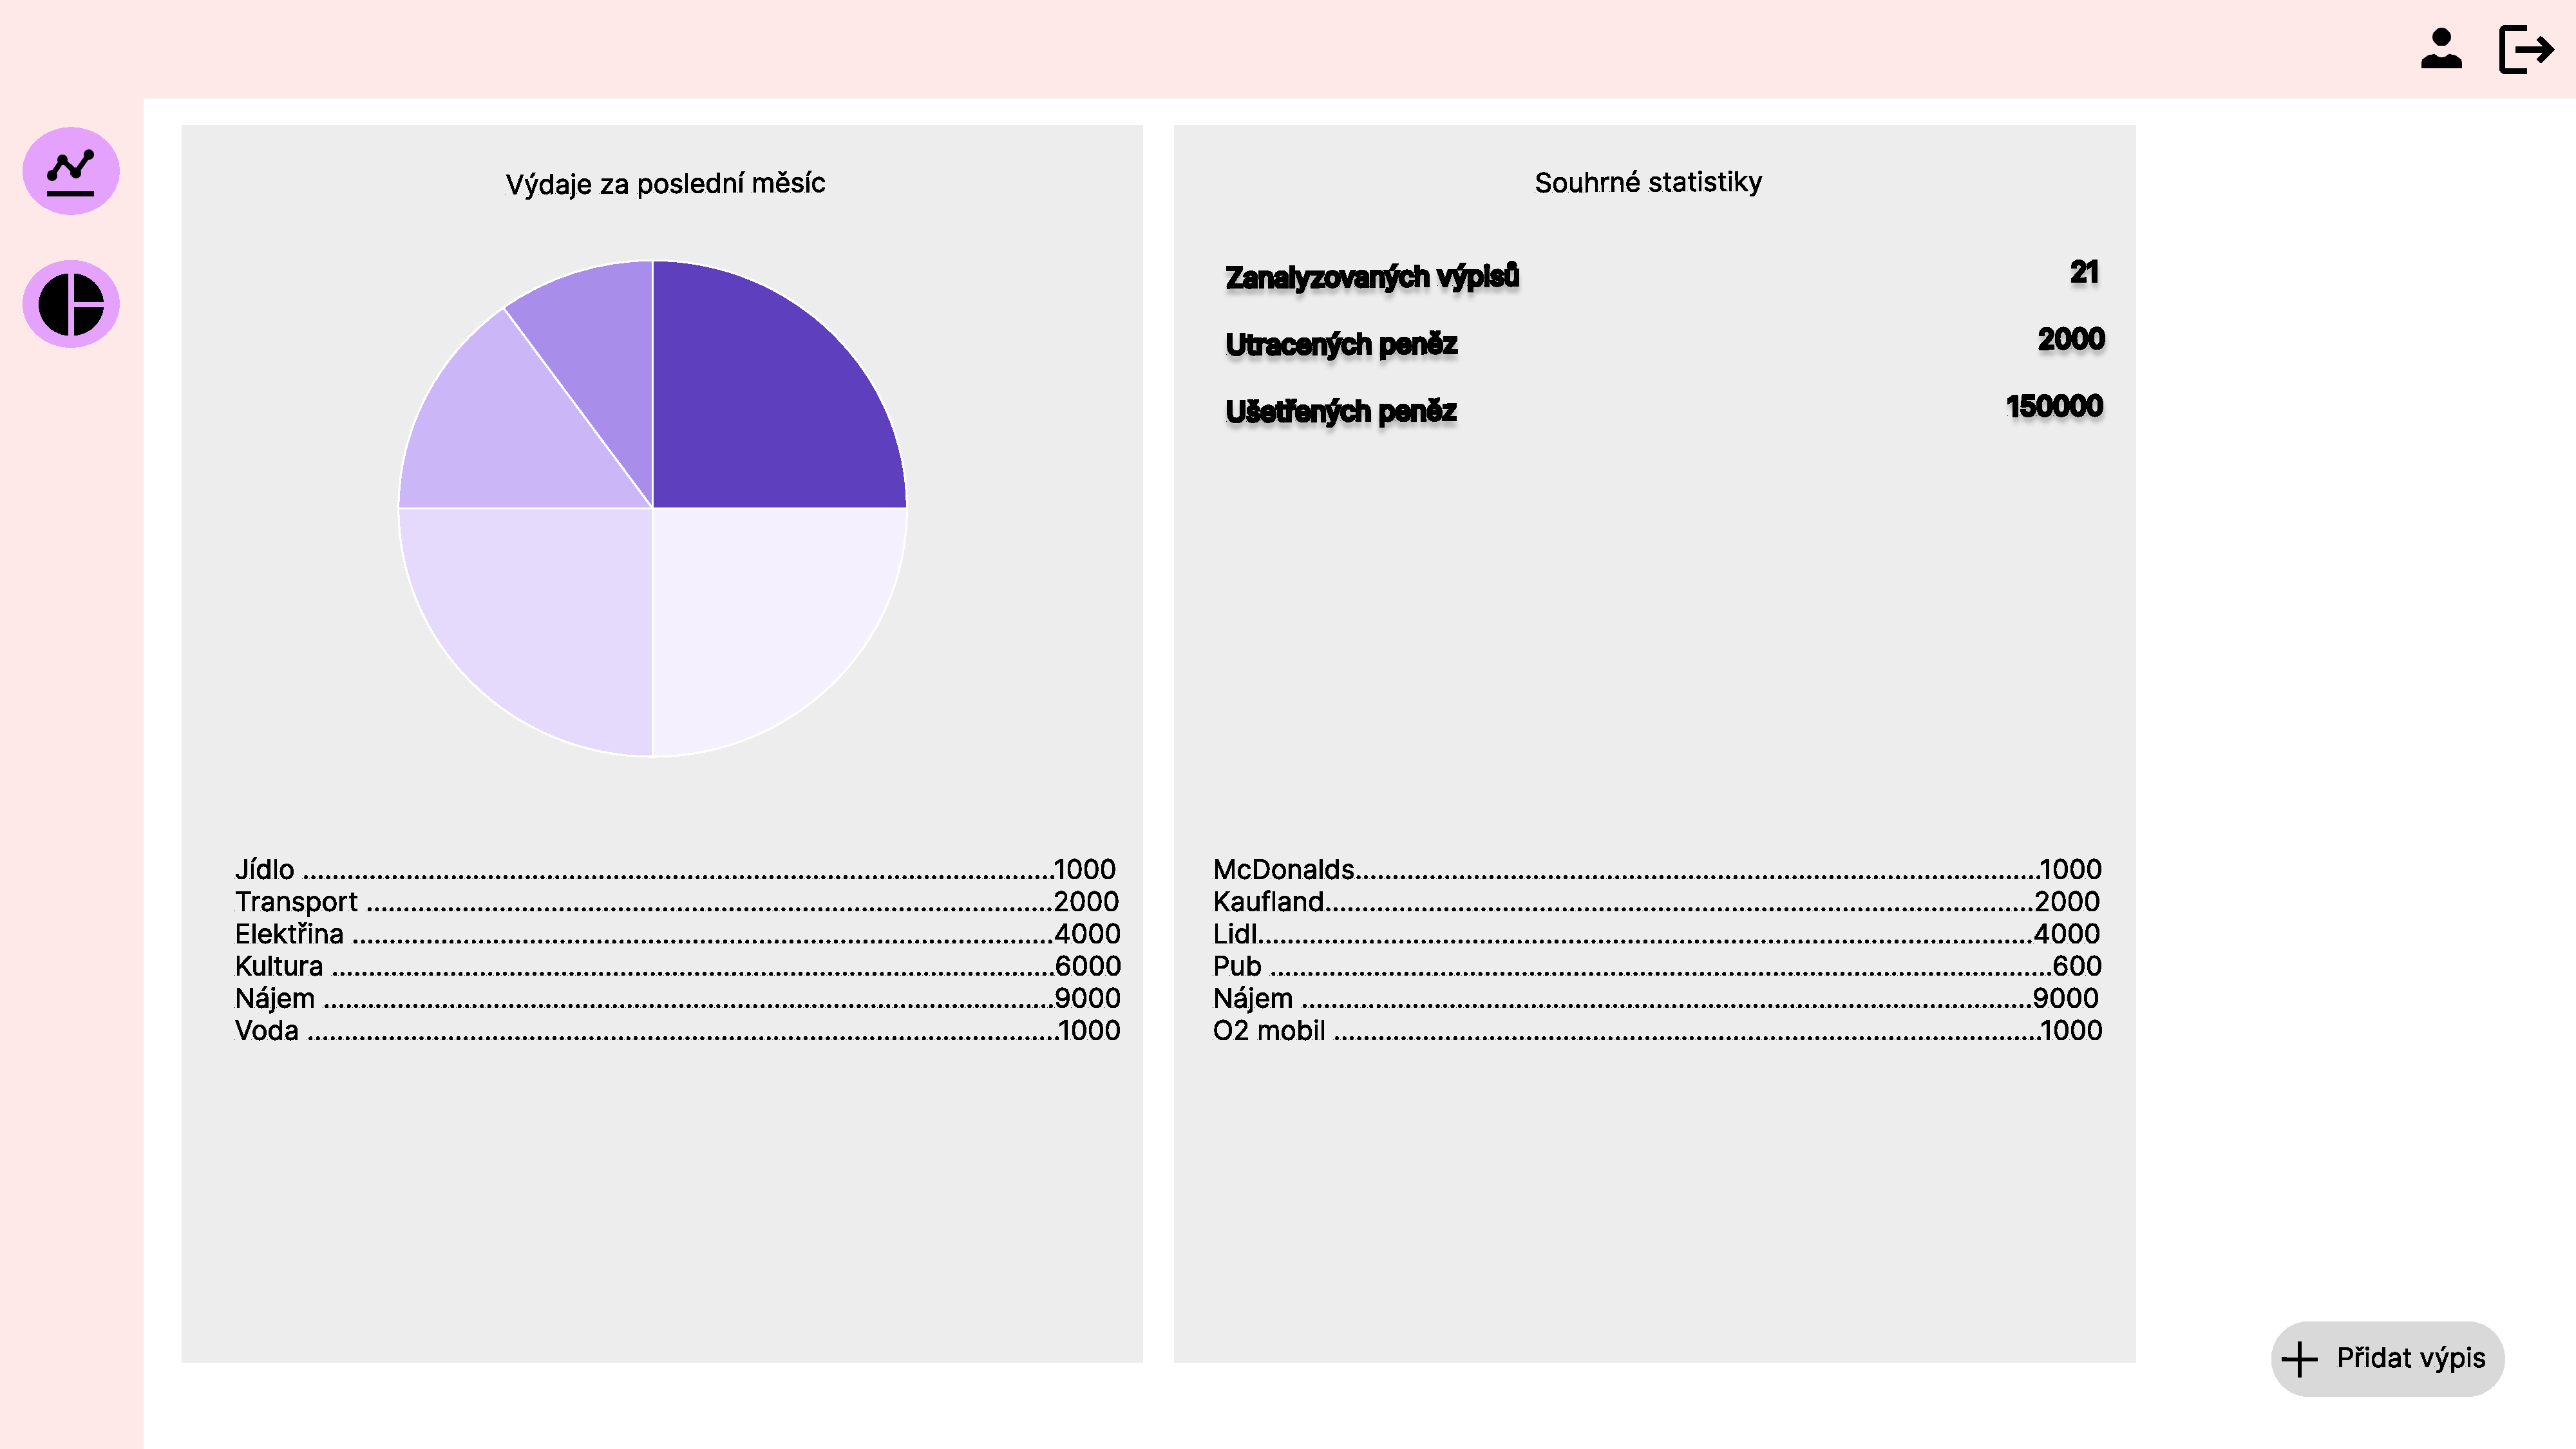
\includegraphics[width=\textwidth]{obrazky-figures/navhrui1.pdf}
\caption{Wireframe domovské obrazovky.}
\label{fig;wireframe}
\end{figure}

Hlavní a~\uv{úvodní} obrazovka, kterou uživatel uvidí první po přihlášení, bude obrazovka s~analýzou výpisu z~posledního měsíce. Nejsignifikantnějším prvkem bude graf s~barevně rozlišenými kategoriemi. Tady si po pravé straně uživatel bude moct prohlížet a~upravovat transakce z~posledního měsíce. Uživatel bude moci najet myší na graf a~zobrazit přesně, ke~které barvě patří jaká kategorie a~kolik v~ní utratil.
Navigace bude mít 5 nejdůležitějších tlačítek Domů, Výpisy, Grafy, Profil a~Odhlášení. Nejdůležitější tlačítko volající o~akci uživatele bude v~levém dolním rohu \texttt{+ Přidat výpis}. Stisknutím tlačítka uživatel nahraje výpis a~následně spustí analýzu transakcí. To vše v~modálním okně, které bude taky znovu použitelné pro editace transakcí nebo výpisů. Kde ve formuláři bude každé políčko jeden atribut z~ER Diagramu (obrázek \ref{fig:erdiagram}) a~půjde jednoduše upravovat.

Na druhé hlavní obrazovce se statistikou může uživatel pozorovat své finance v~dlouhodobém měřítku. Může usoudit, ve které oblasti je potřeba zlepšit své osobní finanční rozhodování. Bude mít k~dispozici souhrnné grafy za posledních několik měsíců, jak lze vidět na obrázku~\ref{fig;wireframe2}.
\begin{figure}[H]
\centering
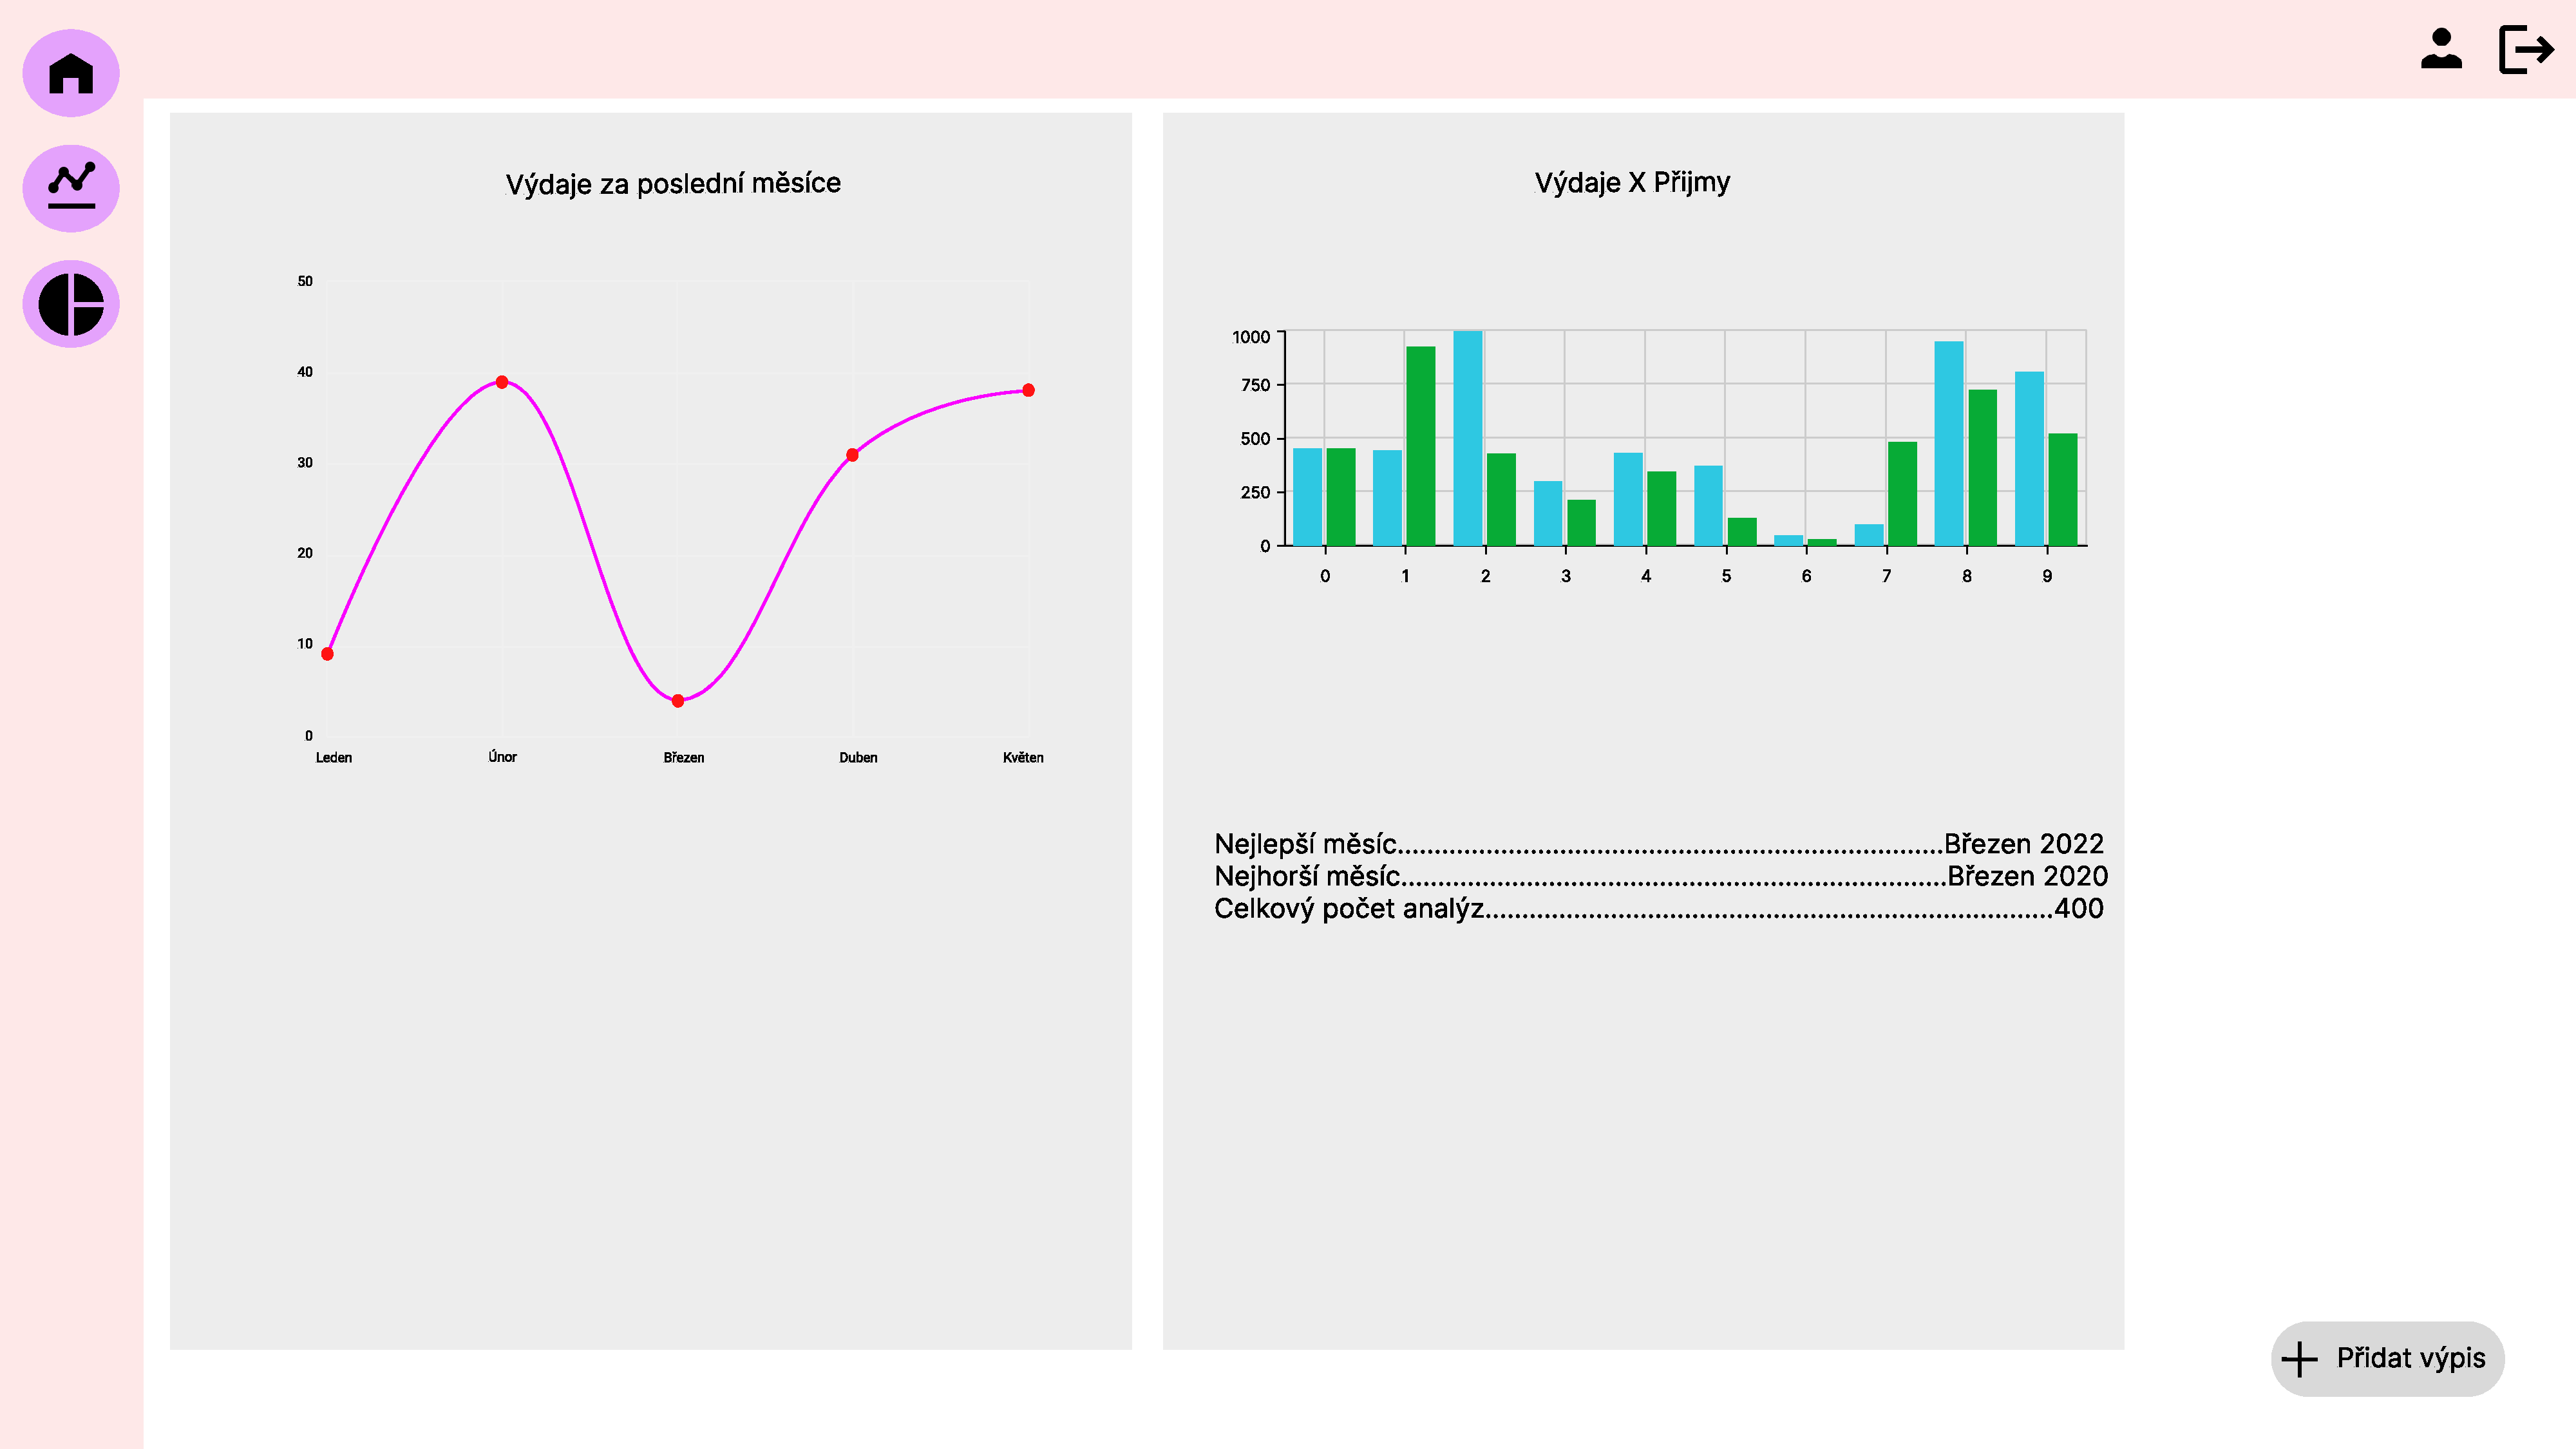
\includegraphics[width=\textwidth]{obrazky-figures/navrhui2.pdf}
\caption{Wireframe obrazovky se statistikou.}
\label{fig;wireframe2}
\end{figure}

\section{Návrh API}
Správný návrh API je klíčovým prvkem při vývoji aplikace a~je nutné se mu věnovat s~dostatečnou pozorností a~pečlivosti. Základní předpoklad pro návrh API je analýza návrhu UI. Zde je potřeba popřemýšlet, jaké datové podklady na které stránce jsou potřeba.
Pro každou entitu je potřeba navrhnout 4 základní HTTP metody. Tyto metody nám poslouží k~vytvoření nové entity, získání dat o~entitě, úpravu entity a~smazání entity. Tento druh endpointů je základ kvalitní aplikace.
Seznam navržených endpointů na serveru, které vyvolávají akci:
 \begin{itemize}
     \item \texttt{GET, POST /user}
     \item \texttt{PUT, DELETE /user/<user\_id>}
     \item \texttt{POST /statement}
     \item \texttt{GET, PUT, DELETE /statement/<statement\_id>}
     \item \texttt{POST /transaction}
     \item \texttt{GET, PUT, DELETE /transaction/<trans\_id>}
     \item \texttt{POST /token}
     \item \texttt{GET /lateststatement}
     \item \texttt{GET /allstatements/}
     \item \texttt{GET /statement/<statement\_id>/transactions}
     \item \texttt{GET /analyze/<statement\_id>}
 \end{itemize}
Pojmenování těchto CRUD endpointů se řídí pravidly REST API. To znamená, že~endpointy~(transakce, výpis) se pojmenovávají dle tohoto klíče. GET, PUT a~DELETE \break \texttt{/<jméno\_entity>/<identifikační\_číslo>} a~POST \texttt{/<jméno\_entity>/}. Na výpisu \ref{lst:httpget} lze vidět jak požadavek a~odpověď vypadají.
\begin{lstlisting}[breaklines=true,caption={Příklad požadavku \texttt{GET /statement/84}.},label={lst:httpget}]
GET http://127.0.0.1:5000/statement/84
{
    "bank": "Komercka",
    "filename": "kb_november.csv",
    "id": 84,
    "income": 40462,
    "month": 12,
    "spending": 40090,
    "type": "Checkings",
    "year": 2022
}
\end{lstlisting}

Pojmenování endopointu pro entitu uživatel je odlišné, protože díky JWT autentizačnímu tokenu v~hlavičce požadavku dokážeme rozeznat uživatele bez potřeby identifikačního čísla umístěného na konci endpointu. Z~tohoto důvodu bude pro metody GET a~POST endpoint pojmenován \texttt{/uzivatel/} a~pro PUT a~DELETE bude pojmenován\break \texttt{/uzivatel/<identifikační\_číslo>}.

Další endpoint \texttt{/token} slouží na získání autentizačního tokenu JWT, který následně vloží klient do hlavičky HTTP požadavku. Tento endpoint je důležitý pro přihlášení a~autentizaci uživatele.

Následuje skupina endpointů \texttt{/lateststatement}, který vrací výpis z~posledního měsíce a~\texttt{/allstatements}, který vrací všechny uživatelovi výpisy, zjištění uživatele lze znova poznat pomocí autentizační hlavičky.
Kombinovaný endpoint dvou entit \break \texttt{/statement/<statement\_id>/transactions} vrací data o~všech transakcích, které daný výpis obsahuje.

Poslední endpoint \texttt{/analyze} nevrací nic, pouze provede na daném výpisu kategorizaci transakcí a~přidá transakce do databáze.


\chapter{Implementace}
V~následující kapitole budou popsány implementační detaily serveru a~klienta.

\section{Implementace serveru}
Server běží na webovém frameworku Flask. Server je rozdělen do několika podsouborů. Hlavní soubor, který tvoří jádro celé aplikace je pojmenovaný \texttt{server.py}, zde běží celé API, a~v~dalších třech souborech běží model umělé inteligence (\texttt{model.py}), extrakce dat z~výpisu (\texttt{template\_analyze.py}) a~kategorizace výpisů 
 bez AI (\texttt{static\_analyze.py}).
 
\subsection{Implementace API}
Flask nabízí jednoduché a~minimalistické vytvoření API. K~rozběhání serveru stačí inicializovat Flask do proměnné \texttt{app} a~následně ji spustit. Pro napojení na databázi potřebujeme Python knihovnu SQLAlchemy\footnote{\url{https://www.sqlalchemy.org/}}. Tato knihovna nám umožní pracovat s~databází v~prostředí Python a~zpřístupní nám možnost vymodelovat databázi. Podobně jako Flask i~SQLAlchemy se musí inicializovat a~následně pracovat pod proměnou \texttt{db}. Pro každou entitu z~ER diagramu vytvoříme třídu s~definicí, jaké atributy má daná třída mít v~databázi. Pro získávání dat z~databáze pomocí dotazů je vytvořena speciální třída se schématem, který je typově stejný jako související třída pro databázový model. Tato třída je z~knihovny Marshmallow\footnote{\url{https://flask-marshmallow.readthedocs.io/en/latest/}} slouží pro deserializaci databázového objektu. To znamená, že díky převodu na schéma je možné rovnou posílat data v~JSON formátu.


Každý endpoint se definuje ve webovém frameworku Flask pomocí \break \texttt{@app.route('/cesta', methods=["POST"])}, zde si může nastavit požadovanou URI a~povolené HTTP metody.

V~metodě GET pomocí knihovny SQLAlchemy je vytvořen hledací dotaz do databáze \break (např. \texttt{User.query.filter\_by(id=user\_id).first()}). Tento příklad vrací objekt User s~hledaným identifikátorem, díky převodu na schéma můžou být informace o~objektu poslány zpět na klienta.

V~metodě POST se odeslaná data z~klienta na serveru přijmou ve formátu JSON. Na serveru se uloží do proměnné pomocí \texttt{request.json} všechny informace z~těla HTTP zprávy. Tato proměnná použije funkci \texttt{data.get('klíč')}. Klíč definuje, která hodnota z~JSON formátu bude vybrána a~uložena. Poté se všechny hodnoty uloží do třídy s~příslušným názvem a~pomocí \texttt{db.session.add('třída')} a~\texttt{db.commit()} se objekt vkládá do databáze.

Metoda PUT operuje podobně jako metoda POST s~tím rozdílem, že se první pokusí najít objekt, který má upravovat v~databázi.

Metoda DELETE pouze vyhledá v~databázi objekt a~příkazem \break \texttt{db.session.delete(objekt)} smaže objekt.
Po každé úpravě databáze musí být volána funkce \texttt{db.session.commit()} pro perzistentní stav databáze.


\subsection{Extrakce dat z~šablony}
Jak jsem již formuloval v~kapitole \ref{chap:formaty}, každá banka má rozdílné výpisy transakcí. Proto je potřeba pro každou banku vytvořit vlastní funkci k~extrakci dat.
\subsubsection{AirBank}
AirBank používá formát CSV v~kódování WIN-1250. Funkce \texttt{Airbank\_analyze()} otevře soubor pro čtení a~pomocí knihovny pro čtení CSV souboru otevře soubor a~hledá požadované sloupečky v~souboru: \uv{Název protistrany} a \uv{Částka v~měně účtu} tyto dvě informace nám stačí pro vytvoření objektu Transakce a~spuštění automatické klasifikace transakce.

\subsubsection{Fio}
Fio nabízí své výpisy v~CSV formátu. Postup je podobný jako u~AirBank. Otevřeme CSV soubor a~hledáme sloupečky v~souboru, které obsahují podrobné informace o~transakci (\uv{Název obchodníka} popřípadě \uv{Poznámka}, \uv{Zaúčtovaná částka}).

\subsubsection{Československá obchodní banka}
ČSOB nabízí výpisy ve formátu XML i~s~jejich detailně popsanou dokumentací\footnote{\url{https://www.csob.cz/portal/documents/10710/1927786/ceb-vypisy-format-xml.pdf}}. Pomocí knihovny XML pro načtení stromové struktury do proměnné postupně procházíme strukturou a~hledáme položky s~tagem \uv{Ntry} pro zjištění, že se jedná o~záznam o~transakci. V~transakci hledáme \uv{Amt} pro zjištění částky a~dále zjišťujeme pomocí tagu \uv{CdtDbtInd} zda je platba kladná (\uv{CRDT}) nebo záporná (\uv{DBIT}). A~po dalším zanoření hledáme \uv{NtryDtls} neboli detail transakce. A~pro samotný popis transakce se musíme zanořit ještě o~dvě úrovně níž na položku \uv{Ustrd}, ze které musíme odstranit lokaci a~částku pro další kategorizaci.

\subsubsection{Moneta}
Moneta taktéž nabízí výpisy ve formátu XML a~poskytuje jejich detailně popsanou strukturu\footnote{\url{https://www.moneta.cz/documents/20143/11740743/mmb-ib-struktura-vypisu-xml.zip}}. Moneta má na rozdíl od ČSOB jednodušší stromovou strukturu a~hledáme pouze elementy s~tagem \uv{transaction}, kde pak hledáme atributy s~názvem \uv{amount} pro částku a~pro popis transakce se zanoříme do \uv{trn-messages} a~následně do \uv{trn-message}. V~tomto bodě zanoření byl nalezen popis transakce a~můžeme spustit automatickou kategorizaci a~uložit objekt do databáze.

\subsubsection{Komerční banka}
Komerční banka poskytuje své výpisy ve formátu CSV. Na rozdíl od ostatních bank přidává do svých výpisů nadstandardně velkou hlavičku, kterou je nutné odstranit. Po analýze několika výpisů od různých lidí se mi potvrdilo, že nejlepší cestou bude otevřít soubor odstranit z~něj prvních 17 řádků, uložit a~až potom ho načíst knihovnou pro čtení CSV. Dále procházíme soubor a~hledáme sloupečky \uv{AV pole 1} a~pole \uv{Částka}. Tato data nám stačí pro přidání objektu Transakce do databáze. Zkusíme spustit automatickou detekci kategorie a~transakci uložíme.

\subsubsection{UniCredit bank}
UniCredit banka poskytuje výpisy ve formátu CSV. Tyto výpisy podobně jako výpisy z~Komerční banky obsahují hlavičku. Proto je nutné  odstranit z~nich prvních 5 řádků, uložit soubor a~až potom jej načíst knihovnou pro čtení CSV. Dále procházíme soubor a~hledáme sloupce \uv{Částka} a~\uv{Příjemce}. Následně spustíme automatické řazení transakcí a~uložíme transakce do databáze.


\subsubsection{Budoucí přidání dalších bank}
\label{chap:addbank}
Budoucí rozvoj aplikace a~přidávání všech českých a~světových bankovních společností je vítaným rozšířením. Největším problémem s~přidáním nové banky je získání dostatečného množství vzorků výpisů z~banky. Bankovní společnosti nebyly nejochotnější v~komunikaci s~poskytnutí testovacích výpisů. Po dostatečné analýze je potřeba pouze vytvořit novou funkci v~souboru \texttt{template\_analyze.py}. Je potřeba vytvořit funkci, která přečte celý soubor, najde příslušné položky ve výpisy (částku, popis transakce), provede kategorizací a~přidá transakci do databáze.


\section{Implementace klienta} 

Klient běží na webovém frameworku React. Celkové rozložení implementace je složeno z~menších komponent, které dohromady tvoří celé stránky v~aplikaci.
\subsection{Použité balíčky}
React má obrovskou komunitní základnu a~proto je k~dispozici mnoho balíčků, které nám s~ním umožní lépe pracovat. V~následujících kapitolách popíši jen ty nejzajímavější.
\subsubsection{Material UI}
Material UI\footnote{\url{https://mui.com/}} je open source knihovna uživatelského rozhraní pro React framework, která poskytuje předdefinované komponenty a~stylizaci v~souladu s~designovým jazykem Material Design od Google\footnote{\url{https://m1.material.io/}}. Material UI přináší rozsáhlou nabídku přizpůsobitelných komponent, zahrnujících tlačítka, formulářová pole, ikony, nabídky a~další prvky, které lze snadno implementovat pro vytvoření moderního, jednotného a~esteticky příjemného uživatelského rozhraní. Tato knihovna nabízí možnosti vysokého stupně flexibility a~přizpůsobení, což umožňuje vývojářům snadno upravit vzhled a~funkčnost komponent, které zrovna vývojář potřebuje. Knihovna disponuje skvěle zpracovanou dokumentací, což představuje jednu z~hlavních faktorů, proč jsem se rozhodl ji využít.

\subsubsection{Axios}
Axios\footnote{\url{https://www.npmjs.com/package/axios}} je Javascriptová knihovna, která umožňuje vytváření HTTP požadavků v~prostředích s~použitím React frameworku. Tato knihovna poskytuje vývojářům širokou knihovnu funkcí pro získávání a~odesílání dat mezi klientem a~serverem. 

\subsubsection{Toastify}
Toastify\footnote{\url{https://fkhadra.github.io/react-toastify/introduction}} je knihovna pro React, která umožňuje uživatele upozorňovat (tzv. toast zprávou) na různé změny a~události. Tyto upozornění se většinou nachází v~jednom ze čtyř rohů obrazovky.

\subsubsection{Recharts}
Knihovna Recharts\footnote{\url{https://recharts.org/en-US/}} je open--source a~slouží k~vytváření interaktivních grafů. Knihovna nabízí mnoho různých typů grafů, jako jsou liniové grafy, sloupcové grafy, koláčové grafy, časové osy a~další. Stala se velmi populární hlavně z~důvodů obrovské možnosti přizpůsobení grafů (např. barvy, šířku čar, styl os atd.).

\subsection{Komponenty}
Dle návrhu je práce rozdělena na několik menších stránek. Každá stránka se skládá ze samostatné komponenty nebo z~více komponent. 
Ve složce \texttt{src/componenets} je pro každou komponentu vyhrazen samostatný soubor.
Zajímavější komponenty jsem se snažil rozebrat v~následujících kapitolách.

\subsubsection{App.js}

Funkce \texttt{App} definuje a~inicializuje základní strukturu aplikace. Používá se zde komponenta BrowserRouter, která poskytuje routing pro aplikaci, a~inicializuje komponentu ToastContainer, která bude zobrazovat zprávy pro uživatele v~rámci celého prostředí aplikace. Routing pro aplikaci znamená, že vytvoří cesty pro jednotlivé stránky, aby měla každá stránka svou URL.
\subsubsection{UseToken.js}

Tato komponenta pracuje hlavně s~JWT tokenem. Obsahuje tři funkce \texttt{getToken}, \texttt{saveToken} a~\texttt{removeToken}. Funkce \texttt{saveToken} uloží JWT token do Local Storage a~pokud bude klient posílat další požadavky bude token jednoduše získatelný. Funkce \texttt{getToken} dokáže získat uložený JWT token z~Local Storage a~znovu ho použít při dalším HTTP požadavku. Funkce \texttt{removeToken} odstraní z~Local Storage token a~tím se uživatel nemá jak autentizovat při dalším HTTP požadavku.
\subsubsection{Login.js}

Je jedna z~nejdůležitějších komponent aplikace, zde se uživatel autentizuje do aplikace. Uživatelovi se zobrazí formulář pro zadání svých inicializačních údajů. Pomocí zadání své emailové adresy a~hesla, a~následným kliknutím na tlačítko \texttt{Sign in}, odešle klient pomocí Axios knihovny HTTP požadavek, který vrátí autentizační token. Pokud server vrátí úspěšnou odpověď na požadavek, přesměruje se klient na stránku \texttt{Home.js}. V~případě, že autentizace selže, dojde k~resetování polí pro zadání údajů a~zobrazení zprávy o~neúspěchu.

\subsubsection{Home.js}
Domovská obrazovka, jak z~návrhu vyplývá, je první obrazovka se kterou se setká uživatel. Vnitřní logika volá endpoint pro získání dat z~posledního výpisu a~následuje endpoint na všechny transakce daného výpisu. Tato data dále posílá jako argumenty do dalších komponent. Na obrázku \ref{fig:homescreen} lze vidět rozdělení na 4 komponenty -- Navigační lišta (\texttt{NavBar}), Nahrávání výpisu (\texttt{Upload}), Výpis transakcí (\texttt{Transaction}) a~Výsečový diagram (\texttt{Graph}). 

\begin{figure}[ht]
    \centering
    \includegraphics[width=\textwidth]{obrazky-figures/moneyhome.png}
    \caption{Domovská obrazovka aplikace.}
    \label{fig:homescreen}
\end{figure}

\subsubsection{Transaction.js}
Transactions zobrazuje tabulku všech transakcí, které jsou předány jako argument. Pomocí mapovací funkce \texttt{transaction.map()} se tabulka rozšíří nebo zmenší na základě poskytnutých dat. Tabulka zobrazí všechny důležité parametry entity Transakce. Uživatel může díky ikonám rychle upravovat jednotlivé transakce v~modální okně nebo je rovnou smazat.

\subsubsection{Graph.js}
Komponenta obsahuje funkci \texttt{countAmountByCategory}, která vezme data z~transakcí a~spočítá sumu za jednotlivé kategorie, které se nachází v~datech. Funkce data připraví do formátu \texttt{kategorie:částka}, aby je mohla knihovna \texttt{Recharts} použít. Tato data se potom zobrazí v~barevném grafu. 
Tato komponenta se zobrazuje Graf na základě dat transakcí, které komponenta dostane jako argument. 

\subsubsection{Upload.js}
Tato komponenta dovolí uživatelovi nahrát soubor. Po kliknutí na tlačítko \texttt{Upload} se soubor pomocí POST požadavku odešle na server a~pokud přijde kladná odpověď, klient si uloží identifikační číslo výpisu. Uživatelovi se zobrazí modální okno s~požadavkem na vyplnění dodatečných údajů, které se pomocí PUT požadavku pošlou zpět na serveru a~začne analýza transakcí. Dokud není hotova uživatel vidí načítací kolečko, jakmile klient přijme kladnou odpověď serveru přesměruje klienta na detail výpisu.
\begin{figure}[H]
    \centering
    \includegraphics[width=7cm]{obrazky-figures/moneymodalwindow.png}
    \caption{Modální okno pro doplnění informací o~výpisu.}
    \label{fig:statements}
\end{figure}


\subsubsection{Graphs.js}
Stránka s~přehlednými grafy je schovaná v~komponentě \texttt{Graphs.js}. Zde se kromě Navigační lišty nachází dva grafy, jeden zobrazující porovnání příjmů a~výdajů v~průběhů měsíců v~daném roce. Na druhém grafu se zobrazuje křivka výdajů. Pomocí komponenty YearCalendar, která při změně vybraného roku vždy pošle nový požadavek na server a~znovu načte dotčené komponenty, může uživatel měnit časové rozmezí pro data v~grafu.
\begin{figure}[H]
    \centering
    \includegraphics[width=\textwidth]{obrazky-figures/moneygraphs.pdf}
    \caption{Obrazovka pro sledování výdajů v~čase.}
    \label{fig:graphs}
\end{figure}


\subsubsection{Profile.js}
Tato stránka umožní uživateli upravit svůj profil, pomocí komponenty TextField z~Material UI. Předtím než uživatel bude moct data upravovat je zavolán endpoint \texttt{GET /user}, ten nám zajistí nahrání dat do formulářových polí. Uživatel může upravovovat všechny položky, které obsahuje entita Uživatel. Tlačítko vyvolá akci \texttt{SubmitPut}, tato akce zkontroluje zda heslo bylo upraveno a~zkontroluje zda bylo zadáno dvakrát. Tato kontrola je důležitá z~důvodu velice častých chyb, které může uživatel udělat. Následně odešle požadavek\break \texttt{PUT /user/<identifikační\_číslo>} a~klient zobrazí dle odpovědi serveru kladnou nebo zápornou zprávu. Na obrázku \ref{fig:profile} lze vidět úpravu jednoho z~uživatelů.

\begin{figure}[H]
    \centering
    \includegraphics[width=\textwidth]{obrazky-figures/moneyprofile.png}
    \caption{Obrazovka pro úpravu uživatele.}
    \label{fig:profile}
\end{figure}

\subsubsection{Statements.js}
Uživatel využije tuto komponentu při zobrazování detailu jednoho určitého výpisu. Komponenta načítá data z~endpointu \texttt{/allstatements/}. Po načtení dat jsou zobrazeny v~tabulce, kde každý řádek odpovídá jednomu bankovnímu výpisu a~zahrnuje informace o~měsíci, roce, bance, typu, příjmu a~výdajích. Kliknutím na tlačítko \texttt{Edit} v~řádku daného bankovního výpisu se otevře dialogové okno s~editačním formulářem, který umožňuje změnit údaje v~daném záznamu. Po změně údajů je možné uložit změny na server pomocí tlačítka, které volá na endpoint \texttt{/statement/<identifikační\_číslo>}.




\chapter{Automatická klasifikace transakcí}
Různé banky nabízí různé formáty výpisů, jak jsem již uvedl v~kapitole \ref{chap:formaty}, a~tak pokud je chceme automaticky kategorizovat, je potřeba extrahovat stejná data z~každého výpisu. Nejdůležitějším parametrem je \uv{Popis transakce} (v~každé bankovní společnosti se tento parametr nazývá jinak např. \uv{Zpráva} nebo \uv{AV Pole 1} atd.). Tento parametr poskytuje mnoho užitečných informací, jako je jméno příjemce nebo název společnosti, který lze využít pro další kategorizaci.

\section{Python knihovny}
Automatická kategorizace pomocí umělé inteligence se neobejde bez doplňujících knihoven. V~následujících kapitolách si některé upřesníme k~čemu budou použity.
\subsection{PyTorch}
PyTorch\footnote{\url{https://pytorch.org/}} je framework pro strojové učení, který byl vyvinut především pro výzkum v~oblasti umělé inteligence a~neuronových sítí. Tato knihovna umožňuje vývojářům vytvářet a~trénovat složité neuronové sítě. Tuto knihovnu jsem si zvolil pro její vysokou flexibilitu a~efektivitu. PyTorch je základem pro další knihovny, které dále budu používat.

\subsection{Sentence Transformer}
Sentence Transformer je nadstavba pro framework PyTorch, která dokáže vytvořit reprezentaci vět, textů a~obrázků. Tento nástroj lze použít pro výpočet vektorů vět pro více než 100 jazyků, a~poté pomocí kosinové podobnosti porovnat věty s~podobným významem. Tato funkce je užitečná pro sémantické hledání podobností, sémantické vyhledávání nebo hledání parafrází. Nabízí spoustu předtrénovaných modelů a~pro moji práci zvolíme model \textsc{paraphrase-multilingual-mpnet-base-v2}, který byl vytrénován na vícejazyčném datasetu a~je tak vhodný i~na práci s~češtinou~\cite{sentencetransformer}.
Tento model slouží k~vytvoření vektorových reprezentací textu pomocí metody zvané \uv{sentence embedding}. Tato metoda umožňuje převést celou větu nebo odstavec na jednorozměrný vektor, který reprezentuje její sémantický obsah. Tento vektor obsahuje informace o~významu a~kontextu celé věty.
\subsubsection{Kosinová podobnost}
Kosinová podobnost je míra podobnosti dvou vektorů, která se získá výpočtem kosinu úhlu těchto vektorů~\cite{waelhgomaa_2013_a}. Tímto vektorovým porovnání dokážeme rozeznat podobnost jednoho textu k~dalšímu.

\subsection{Pandas}
Pandas\footnote{\url{https://pandas.pydata.org/}} je knihovna pro jazyk Python, která umožňuje efektivní zpracování dat. Knihovna pandas nabízí nástroje pro načítání, manipulaci a~analýzu dat v~různých formátech, včetně CSV, Excel, SQL databází a~mnoha dalších. Tato knihovna nám ulehčí práci při načítání datasetu pro trénování umělé inteligence.

\subsection{Natural Language Toolkit}
Natural Language Toolkit\footnote{\url{https://www.nltk.org/}} (NLTK) je knihovna pro jazyk Python, která umožňuje snadné zpracování a~analýzu přirozeného jazyka. NLTK poskytuje nástroje pro tokenizaci, stemming, lemmatizaci, syntaktickou analýzu a~mnoho dalších úloh v~oblasti zpracování textu. V~mé práci ji hlavně využijeme na tokenizaci textu.

\subsection{Bidirectional Encoder Representations from Transformers}

Bidirectional Encoder Representations from Transformers (BERT) je jazykový model pro strojové učení, který vytvořila společnost Google. Jedná se o~naučený model založený na architektuře transformátorů, který se specializuje na zpracování přirozeného jazyka. BERT je schopen provádět širokou škálu úloh, jako je například klasifikace textu, zodpovídání otázek, generování textu a~mnoho dalších~\cite{bertcitace}.
BERT s~knihovnou Sentence Transformer budou posuzovat podobnost transakcí.

\section{Implementace modelu AI}
Implementace modelu na serveru se inspiruje z~\cite{cuicategorize}.
Na serveru je modelu AI dedikován celý soubor \texttt{model.py}. Tento soubor nejdříve načte data a~funkce \texttt{clean\_text\_bert} je následně očistí od zbytečných znaků a~celou transakci promění na tokeny, které poté lépe dokáže zpracovat model.
Poté následuje inicializace modelu z~knihovny SentenceTransformer s~názvem \texttt{paraphrase-multilingual-mpnet-base-v2}. Dále se vytvoří vektorové reprezentace textu pro vstupní data. Výsledkem je objekt \texttt{embeddings}, který obsahuje vektorové reprezentace textu. 
\begin{lstlisting}[language=python,caption={\texttt{model.py}.},label={lst:modelpy},breaklines=true]
    df = pd.read_csv('dataset.csv')
    text_raw = df['Transaction']
    text_BERT = text_raw.apply(lambda x: clean_text_BERT(x))
    bert_input = text_BERT.tolist()
    model = SentenceTransformer('paraphrase-multilingual-mpnet-base-v2')
    embeddings = model.encode(bert_input, show_progress_bar=True)
    embedding_BERT = np.array(embeddings)
\end{lstlisting}
Při tvoření objektu transakce se volá funkce \texttt{ai\_categorization(text)}. Funkce spustí model umělé inteligence a~ten pomocí kosinové podobnosti a~jazykového modelu BERT se pokusí najít dle kontextu slov podobnou transakci z~datasetu a~pomocí této transakce se určí kategorie pro transakci. Zkrácenou verzi funkce můžeme vidět na výpisu~\ref{lst:aicategorizace}.
\begin{lstlisting}[language=python,caption={Funkce \texttt{ai\_categorization(text)}.},label={lst:aicategorizace},breaklines=true] 
def ai_categorization(transaction_text):
    data = [transaction_text]
    df_test = pd.DataFrame(data, columns=['Test'])
    text_test_raw = df_test['Test']
    text_test_BERT = text_test_raw.apply(lambda x: clean_text_BERT(x))
    bert_input_test = text_test_BERT.tolist()
    embeddings_test = model.encode(bert_input_test, show_progress_bar=True)
    embedding_BERT_test = np.array(embeddings_test)
    df_embedding_bert_test = pd.DataFrame(embeddings_test)
    similarity_new_data = cosine_similarity(embedding_BERT_test, embedding_BERT)
    similarity_df = pd.DataFrame(similarity_new_data)
    data_inspect = df.iloc[index_similarity, :].reset_index(drop=True)
    category = data_inspect['Category']
    return category[0]
\end{lstlisting}

\section{Trénování modelu}

Pro správnou funkčnost kategorizace je potřeba natrénovat model pro umělou inteligenci na nějakém vhodném datasetu. 
\\
Vyextrahoval jsem své osobní transakční data z~banky a~také data od rodinných příslušníků a~kamarádů. Takto vznikla kolekce dat, která obsahuje více než 5000 transakcí. Z~transakcí jsem použil pouze sloupeček s~popiskem transakce. Z~mé datové analýzy jsem se dozvěděl, že supermarkety nemají stejná čísla bankovního účtu jako stejná značka supermarketu v~jiném městě. 
\\
Rozhodl jsem se rozdělit transakce na tyto kategorie:
\begin{itemize}
    \item \textbf{Potraviny}
    \item \textbf{Oblečení}
    \item \textbf{Pravidelné výdaje} -- Energie, elektřina, voda, topení, splátky, hypotéky, nájem
    \item \textbf{Investice} -- Investiční výdaje a~odkládání peněz na spořící účet
    \item \textbf{Transport} -- Jízdenky a~MHD
    \item \textbf{Internetové nákupy} -- Jakákoliv transakce, která prošla přes internetovou platební bránu
    \item \textbf{Palivo} -- Benzín, nafta
    \item \textbf{Přeposílání peněz} -- Převod peněz na další účet, nebo dobití peněz na Revolut
    \item \textbf{Bankomat} -- Výběr peněz z~bankomatu 
    \item \textbf{Mobil} -- Dobíjení kreditu, placení paušálu
    \item \textbf{Nákupy} -- Všechno ostatní co nepatří do potravin a~oblečení
    \item \textbf{Předplatné} -- Noviny, časopisy, hudební a~streamovací služby
    \item \textbf{Lékárna} -- Léky
    \item \textbf{Zábava} -- Lístky na představení, bar nebo výlety    
\end{itemize}

Testovací data obsahují 100 transakcí z~čehož se zde nachází, jak transakce známé v~datasetu tak i~neznámé. Známé transakce se zde nacházejí pro kontrolu správnosti.

V~následujících kapitolách popíšu experimenty, které jsem provedl a~který postup jsem nakonec zvolil do výsledné aplikace. 
\subsection{Trénovaní modelu na nevyčištěných datech}
Neošetřená data obsahují mnoho záznamů, která jsou duplicitní, prázdná nebo nesmyslná pro potřeby trénovaní modelu např. obsahují směs znaků a~číslic ze které nedokážeme vyvodit kategorii transakcí. Po této selekci transakcí jsem se dostal na číslo 400 použitelných transakcí. Transakce jsem ručně prošel a~přidal k~ním výše zmíněnou kategorii do které patří. Pokud jsem nedokázal posoudit kam transakce patří, zařadil jsem ji do kategorie Neznámé.



Po provedení experimentu jsem došel k~závěru, že tato metoda nedává nijak obstojné výsledky a~ze 100 transakcí bylo správně rozpoznáno 63 transakcí (z~toho 40 bylo předem známých, 23 neznámých) a~37 transakcí bylo nepřesně zařazeno nebo zcela mimo obor (10 předem známých, 27 neznámých). Z~trénovaní vyšlo najevo, že největší problém dělají umělé inteligenci jména a~adresy, pokud je v~popisku transakce pouze jméno, nedokáže najít přesnou shodu a~pokud je tam jenom adresa, tak z~toho taktéž nelze určit o~co se jedná. Častá chyba umělé inteligence byla, že se snažila přiřadit kategorii dle místa.
Konečná úspěšnost je 80 \% na známých transakcích a~46 \% na nových. Z~těchto čísel se dá spočítat kombinovaná úspěšnost 63 \%.

Příklady chybně kategorizovaných transakcí lze vidět v~tabulce \ref{tab:exp1}.

\begin{center}
\begin{table}[h]
\centering
\begin{tabular}{ |c| c| c| }
\hline
\textbf{Nová transakce} & \textbf{Odpovídající transakce}  & \textbf{Kategorie} \\  
\hline
ZHU TE MIAO & JIZDNE   *UHBUkf1549 & Transport \\ 
\hline
KB ATM UH.BROD KAUFL & Sklizeno & Potraviny  \\ 
\hline
DECATHLON ZLIN & MCD Zlin & Jídlo  \\  
\hline
MOBELIX BRNO SPLAVIS & MOL - BRNO - 606 & Palivo  \\
\hline
HRACKY SOUKENIK & JIZDNE   *UHBUmi1925 & Transport  \\
\hline
\end{tabular}
\caption{Příklady chybných transakcí v~experimentu č.1}
\label{tab:exp1}
\end{table}
\end{center}

\subsection{Trénovaní modelu na vyčištěných datech}
V~minulém experimentu jsem zaznamenal vysokou chybovost v~datech, které nejsou očištěné např. \uv{Tesco Brno} a~\uv{McDonalds Brno} (obě byly zařazeny do kategorie Potraviny). V~tomto případě chybně rozezná kategorii a~přiřadí ji podle města. Tento jev je chybný. Dalším problémem jsou čísla transakcí a~různé další klasifikátory v~popiscích transakcí (např.~\uv{Revolut x4564d}). V~tomto trénování modelu očistíme dataset od všech nepotřebných informací o~transakci, jako jsou čísla objednávek a~město, ve kterém se platba uskutečnila. Do datasetu jsem také přidal nejznámější obchodní řetězce působící v~České republice a~přiřadil k~nim jejich kategorii. V~tomto experimentu se špatně rozdělují transakce na již známé a~na úplně nové, neboť pro ošetřené transakce neexistuje stejná transakce v~testovacích datech, ale i~přes tuto skutečnost můžeme porovnat celkovou úspěšnost. 
Po nacvičení modelu vyšla následující úspěšnost. Ze 100 testovacích transakcí bylo správně rozpoznáno 69 transakcí a~31 zcela špatně. Toto trénování dosahovalo mnohem lepších výsledků v~oblasti adres, kde již nespojovala dvě transakce jenom podle lokace. 
Příklady chybně kategorizovaných transakcí lze vidět v~tabulce \ref{tab:exp2}.
Z~toho výsledku můžeme usoudit, že jsme dosáhli skoro 70\% úspěšnosti. Proto je vhodné s~tímto modelem pokračovat dále.

\begin{center}
\begin{table}[h]
\centering
\begin{tabular}{ |c| c| c| }
\hline
\textbf{Nová transakce} & \textbf{Odpovídající transakce}  & \textbf{Kategorie} \\  
\hline
ENFIN CZ A.S. & NOTINO & Nákupy \\ 
\hline
HANACKA HOSPODA  & Zasilkovna & Nákupy  \\ 
\hline
PRIMARK PRAGUE & Bageterie Boulevard  & Jídlo  \\  
\hline
SHELL 8014  & Revolut & Převod peněz  \\
\hline
KAUFLAND CZ  2010 & kfcrozvoz.cz & Jídlo  \\
\hline
\end{tabular}
\caption{Příklady chybných transakcí v~experimentu č.2}
\label{tab:exp2}
\end{table}
\end{center}

\subsection{Kategorizace bez AI}
V~předchozích experimentech byl celý systém založen na umělé inteligenci. V~této kapitole se však snažím přistoupit k~této problematice jiným způsobem. Z~velkého objemu transakcí vyberu ty nejčastěji se vyskytující a~přidám k~ní také seznam obchodním řetězců v~České republice a~vytvořím sadu pravidel. Z~dat jsem dokázal vytvořit přes 200 pravidel, které obsahují ty nejčastěji používaná slova. Pokud část transakce bude obsahovat dané slovo, tak ho můžeme zařadit do dané kategorie. Zde nastává problém, pokud v~transakci nenajdeme slovo, které by spustilo dané pravidlo, tak transakce spadne do kategorie Neznámé. Tento způsob se nedá dobře otestovat na daném testovacím vzorku, protože dopředu budeme vědět výsledek na základě daných pravidel. Tento způsob by se dal využít jako přídavná vrstva pro automatickou kategorizaci.

\subsection{Kombinace AI a~pravidel}
V~minulém experimentu jsem zmínil využití více vrstev pro kategorizaci transakcí. První detail transakce necháme projít pravidly, které jsem zmínil v~minulé kapitole a~poté použiji model AI z~druhého experimentu a~vzniknou nám dvě vrstvy, jak je ukázané na diagramu (obrázek~\ref{fig:vrstvenaimplementace}).
Z~teoretického hlediska by tato kombinace měla přinést nejvyšší úspěšnost a~eliminovat chyby umělé inteligence u~předem známé transakce.
\begin{figure}[H]
\centering
\includegraphics[width=\textwidth]{obrazky-figures/vrstvy.pdf}
\caption{Vrstvená implementace kategorizace.}
\label{fig:vrstvenaimplementace}
\end{figure}
Z~experimentu vyšlo najevo následující: Pokud použijeme testovací sadu, úspěšnost je velmi dobrá, neboť z~původních transakcí se hodně obchodních společností opakuje a~tak už byly zařazeny do pravidel. Můžeme říct, že pokud část transakce byla v~pravidlech, je úspěšnost 100 \%, pokud transakce nebyla kategorizována pravidly, je úspěšnost 70 \%. Z~toho vyplývá kombinovaná úspěšnost 85 \% ve dvouvrstvé architektuře. Uvažujeme, že v~běžném výpisu je průměrně 20-25 \% transakcí, kterou nerozezná systém pravidel a~pouze v~těchto případech bude potřeba spouštět model umělé inteligence. Tyto data jsem dostal po datové analýze mých testovacích výpisů.

\subsection{Závěr}
Po provedení těchto tří experimentů jsem došel k~závěru, že nejlepší je použit dvouvrstvou architekturu, protože předchozí experimenty ukázaly, že použití umělé inteligence ke kategorizaci transakcí nedávalo uspokojivé výsledky. V~prvním experimentu měl model obtíže s~identifikací správné kategorie, zejména pokud byl v~popisu transakce uveden pouze název nebo adresa. V~druhém experimentu, i~když si model vedl lépe po vyčištění dat, stále docházelo k~chybám při klasifikaci transakcí na základě místa. Z~experimentů vyšlo najevo, že dvouvrstvá architektura nám zajistí nejlepší výsledky a~zároveň server bude méně zatížen tím, že se nebude muset tak často provádět výpočet podobnosti v~modelu umělé inteligence.

Při každém experimentu jsem si vedl poznámky k~tomu, která kategorie byla nejčastěji špatně zařazena. Při prvním experimentu se nejčastěji netrefil u~kategorie Nákupy. V~této kategorii chyboval celkově 8krát. Ve druhém experimentu byly nejčastěji chybně zařazeny transakce kategorie Nákupy (8krát). Na rozdíl od prvního experimentu zde se zdvojnásobila chybovost u~kategorie Potraviny. Můžeme konstatovat, že pokud model nevěděl, zkoušel neznámé položky zařadit mezi kategorie, které byly zastoupeny v~datasetu častěji. Na základě těchto informací víme, že model se po úpravě datasetu choval víc předvídavě a~nesnažil se výsledky více roztrousit jak tomu bylo u~prvního experimentu. Toto chování by mohlo být považováno za významné zlepšení, neboť v~případě, že v~rámci transakce není správně rozpoznán význam určitého slova, existuje vysoká pravděpodobnost, že tato transakce spadá do kategorie nákupů či potravin, kde se vyskytuje mnoho malých prodejců.
    
\chapter{Testování}
Testování softwaru je důležitý proces při vývoji softwarových aplikací. Jeho účelem je ověřit, zda aplikace funguje tak, jak by měla, a~zda splňuje požadované specifikace a~funkční požadavky~\cite{singh2012software}. V~následujících kapitolách rozeberu jakým způsobem byla aplikace testována.
\section{Testování API}
Testování probíhalo pomocí aplikace Postman\footnote{\url{https://www.postman.com/}}. Tato aplikace umožňuje vývojářům snadno otestovat API a~získat informace o~jeho funkcích a~chování. Tato aplikace mně velmi pomohla ve zjištění, jak má API správně fungovat a~reagovat na různé požadavky. Aplikace umožňuje si předpřipravit všechny endpointy a~při každé změně v~API jedním kliknutím vyzkoušet, zda jejich odpověď odpovídá změně chování, která byla provedena. Tímto způsobem probíhalo testování API po celou dobu vývoje.
\section{Testování šablon}
Aktuálně aplikace podporuje 5 českých bank (Komerční banka, ČSOB, Moneta, AirBank, Fio). Testovací výpisy pro tyto banky se mně podařilo získat od třech na sobě nezávislých osob pro každou banku. Provedl jsem analýzu výpisu a~zaměřil se na to jak nejlépe vyextrahovat data z~těchto šablon. Následně probíhalo testování na testovacích výpisech, výpisy ve všech třech vydání se shodovali ve své specifikaci a~tak bylo testování úspěšné.
\section{Uživatelské testování}
Uživatelské testování probíhalo ve třech experimentech. Podmínkou pro účast v~testování bylo vlastnit účet u~jedné z~podporovaných bankovních společností. Podařilo se mi najít 3 testovací subjekty, každý tvořil zástupce ze své věkové kategorie (18--30 let, 30--50 let, 50+ let). Testovací subjekty jsem označil jako Testovací subjekt 1 (18--30 let), Testovací subjekt 2 (30--50 let) a~Testovací subjekt 3 (50+ let).
\subsection{Experiment č.1}
V~prvním experimentu měly testovací subjekty za úkol: Vytvořit si účet a~nahrát výpis z~minulého měsíce. U~testovacích subjektů 1 a~2 jsem nenarazil na žádnou chybu a~vše probíhalo hladce. Oba si přirozeným způsobem vytvořili účet a~nahráli své výpisy, které si dopředu stáhli z~internetového bankovnictví. U~třetího testovacího subjektu byl mírný problém s~jazykovou bariérou aplikace je celá v~angličtině a~tak starší člověk může mít problém s~jazykem, po vysvětlení základních slovíček již bylo vše v~pořádku a~experiment pokračoval. Nakonec i~třetí testovací subjekt zvládl dokončit úkol.
Na základě výsledku experimentu lze konstatovat, že experiment lze považovat za úspěšný a~základní úkol aplikace můžeme charakterizovat jako snadno zvládnutelný, jak potvrzují výsledky úspěšného absolvování úkolu všemi třemi testovacími subjekty.
\subsection{Experiment č.2}
Druhý experiment spočíval v~upravení dat na profilu a~úpravou měsíce v~daném výpisu. V~tomto experimentu splnil obě části úkolu bez nápovědy pouze testovací subjekt č.1. Následně subjekty 2 a~3 dokázaly bez problému upravit výpis. U~subjektu 2 a~3 nastaly komplikace v~hledání jak upravit profil uživatele. Po asi 2 minutách hledání jsem daným subjektům poradil, kde hledat. Tyto výsledky mě velmi překvapily a~při návrhu jsem očekával, že bude stačit informace \uv{Profile} při najetí na ikonu myší. 
Na základě výsledků druhého experimentu můžeme tvrdit, že umístnění tlačítka pro úpravu profilu není vhodné pro starší ročníky. To by se dalo změnit např. velkým navigačním tlačítkem \uv{Edit Profile}. 
%\subsection{Experiment č.3}
\subsection{Závěr}
Na základě výsledků provedených experimentů lze konstatovat, že základní principy aplikace jsou snadno zvládnutelné. Účastníci první testovací úkol zvládli bez problému, s~výjimkou jazykové bariéry u~staršího uživatele, které však byly úspěšně překonány. V~rámci druhého experimentu bylo zjištěno, že umístění tlačítka pro úpravu profilu není vhodné pro starší uživatele. Tato skutečnost pravděpodobně nezpůsobí nepoužitelnost aplikace jako celku. Celkově lze tedy říci, že aplikace v~uživatelském testování obstála a~plní svůj účel.
\chapter{Závěr}
Cílem práce bylo navrhnout a~vytvořit webovou aplikaci, která bude analyzovat transakce a~řadit je do předem určených kategorií. Hlavní myšlenkou byla snaha pomoci uživatelovi se lépe orientovat ve svých financích. Významným úspěchem v~kategorizaci transakcí je použití přístupu dvouvrstvé architektury, která dosahuje úspěšnosti 85 \%. Před samotným začátkem vývoje proběhla hloubková analýza webových frameworků a~také byly prozkoumány formáty výpisů konkrétních bankovních společnosti. Následovalo hledání vhodného způsobu jak automaticky kategorizovat transakce a~testování různých přístupů k~automatické klasifikaci. Před implementační částí práce jsem provedl návrh celé aplikace pomocí ER diagramu a~Diagramu případů užití. Dále jsem vyvinul aplikaci, ve které si uživatel vytvoří účet a~nahraje své bankovní výpisy. Tyto výpisy zařadí umělá inteligence do různých kategorií a~uživatelovi se zobrazí graf, ve kterém může pozorovat své výdaje v~různých kategorií. Uživatel může procházet již nahrané výpisy a~porovnávat grafy z~různých měsíců.

Práce mi dala nové poznatky ohledně webových frameworků na straně serveru i~klienta a~také jsem se naučil pracovat s~umělou inteligencí v~jazyce Python. Při vývoji byl kladen důraz na jednoduchost a~uživatelskou přívětivost aplikace. Také jsem se snažil zúročit všechny zkušenosti, které jsem získal v~mém studiu.

V~této práci bych chtěl dále pokračovat, protože je zde mnoho věcí ke zlepšení. Nabízí se zde možnost aplikaci obohatit o~co nejvíce bankovních společností jak z~České republiky tak ze zahraničí. Toto vylepšení je snadné na implementaci (kapitola \ref{chap:addbank}), ale časově náročné na získání informací o~struktuře výpisů a~získání testovacích výpisů. Další vylepšení by se nabízelo napojení na API bank, toto by vyžadovalo nastudovaní a~zjištění, které banky nabízí API a~zda by takový přístup byl možný v~ČR, z~důvodů smluvních podmínek bankovních společností. Dále se nabízí rozšíření o~automatické značení opakovaných plateb a~výplat. V~budoucnosti má tato práce šanci se stát oblíbenou nekomerční aplikaci pro masovou společnost. 
\\
Aplikace je dostupná online na \url{moneytracker.petrhybl.com}.